\documentclass[11pt,a4paper]{article}

% ============ Base packages ============
\usepackage{graphicx}
\usepackage{xcolor}
\usepackage{geometry}
\usepackage{amsmath,amssymb,amsthm}
\usepackage{booktabs}
\usepackage{enumitem}
\usepackage{tabularx}
\usepackage{adjustbox}
\usepackage{caption}
\usepackage{subcaption}
\usepackage{tcolorbox}
\usepackage{algorithm}
\usepackage{algpseudocode}
\usepackage{titlesec}
\usepackage{fancyhdr}
\usepackage{setspace}

% ============ Page setup ============
\geometry{a4paper, top=2.5cm, bottom=2.5cm, left=2.5cm, right=2.5cm}
\setlength{\headheight}{14pt}

% ============ Colors ============
\definecolor{accent}{HTML}{1F4E79}
\definecolor{accentlight}{HTML}{2E86AB}

% ============ Section styles ============
\titleformat{\section}{\Large\bfseries\color{accent}}{\thesection}{1em}{}
\titleformat{\subsection}{\large\bfseries\color{accent!85!black}}{\thesubsection}{1em}{}
\titleformat{\subsubsection}{\normalsize\bfseries}{\thesubsubsection}{1em}{}

% ============ Headers / footers ============
\pagestyle{fancy}
\fancyhf{}
\fancyhead[L]{\small\color{accent!70!black}Temporal Attention Neuron (TAN)}
\fancyhead[R]{\small\color{accent!70!black}\thepage}
\renewcommand{\headrulewidth}{0.4pt}
\renewcommand{\headrule}{\hbox to\headwidth{\color{accent!50!black}\leaders\hrule height \headrulewidth\hfill}}

% ============ Paragraph spacing ============
\setlength{\parskip}{0.4em}
\setlength{\parindent}{2em}
\widowpenalty=10000
\clubpenalty=10000
\linespread{1.15}

% ============ Graphics path ============
\graphicspath{{figures/}}

% ============ Bibliography setup ============
\usepackage[numbers,sort&compress]{natbib}
\bibliographystyle{unsrtnat}

% ============ hyperref (load last) ============
\usepackage[
    colorlinks=true,
    linkcolor=accent,
    citecolor=accent!80!black,
    urlcolor=accent,
    bookmarks=true,
    bookmarksnumbered=true,
    unicode=true
]{hyperref}

\hypersetup{
    pdftitle={The Temporal Attention Neuron: A Minimalist Fusion of Transformer Attention and Spiking Neural Dynamics},
    pdfauthor={Li Zexu},
    pdfsubject={Spiking Neural Networks, Temporal Attention, Predictive Coding},
    pdfkeywords={Spiking Neural Networks, Temporal Attention, Predictive Coding, Surprise Gating, Habituation, Neuromorphic Computing}
}

% ============ Custom commands ============
\newcommand{\surprise}{{S_t}}
\newcommand{\history}{{\mathcal{X}_t}}
\newcommand{\attention}{{\boldsymbol{\alpha}_t}}
\newcommand{\activation}{{A_t}}
\newcommand{\membrane}{{h_t}}
\newcommand{\window}{{\mathcal{X}_t}}

% ============ Theorem environments ============
\theoremstyle{plain}
\newtheorem{theorem}{Theorem}[section]
\newtheorem{lemma}[theorem]{Lemma}
\theoremstyle{definition}
\newtheorem{definition}[theorem]{Definition}

\begin{document}

% ============ Title block ============
\begin{center}
    {\LARGE\bfseries\color{accent} The Temporal Attention Neuron: A Minimalist Fusion of Transformer Attention and Spiking Neural Dynamics\par}
    \vspace{0.8em}
    {\small Li Zexu\par}
    \vspace{0.1em}
    {\footnotesize University of Leeds, School of Physics and Astronomy\par}
    \vspace{0.3em}
    {\footnotesize July 2026\par}
\end{center}
\vspace{0.5em}
\hrule height 0.4pt
\vspace{0.8em}

% ============ Abstract ============
\begin{center}
\begin{minipage}{0.92\textwidth}
\small
\noindent\textbf{Abstract}\quad
Contemporary computational neuroscience and deep learning have evolved along two largely disconnected trajectories. Macroscopic deep-learning architectures such as Transformers employ non-Markovian self-attention to model long-range temporal dependencies, yet operate with few biophysical constraints and high computational costs. Microscopic spiking-neuron models such as the Leaky Integrate-and-Fire (LIF) neuron respect physical principles and metabolic efficiency, but their strictly Markovian dynamics limit the extraction of higher-order temporal patterns. This paper proposes the \textbf{Temporal Attention Neuron (TAN)}, a single-neuron model that combines a Boltzmann-weighted temporal attention kernel with neuromodulatory surprise gating on top of a classical leaky integrator. TAN retains the local, Markovian physical substrate of LIF while adding a non-Markovian temporal receptive field driven by a deviation-from-history signal. Our experiments show that habituation, sparse sensory gating under noise, and adaptive niche localization emerge from the dynamics of this system, without any hard-coded adaptation module or pre-programmed navigation algorithm.

The paper presents a complete empirical and theoretical analysis organised in three layers. \textit{Emergent dynamics} (single-neuron and single-agent levels) demonstrate four behavioural phenomena: spontaneous habituation under sustained stimulation, sparse sensory gating under extreme noise, niche capture in a clean gradient, and hovering in a noisy environment that is phenomenologically analogous to \textit{E. coli} chemotaxis. \textit{Experimental evaluation} provides systematic validation across 50 random seeds: TAN achieves lower error than LIF on the two stochastic tasks with very large effect sizes ($p<10^{-30}$, Cohen's $|d|>5$); the two deterministic tasks produce identical trajectories across seeds, so no statistical test is applicable there, but TAN still achieves lower final error. TAN matches trained RNN and GRU baselines on three of four tasks \textit{without any training}; ablation results are consistent with a functional specialization of the three internal modules (surprise, attention, gate); and parameter sweeps show relatively broad performance plateaus over the tested ranges of TAN's unique parameters ($\lambda$, $\beta$). \textit{Dynamical and information-theoretic analysis} provides a mechanism for the observed behaviour: a fixed-point proof shows that the zero-membrane state is an attracting fixed point under sustained constant input; a 2D state-space projection reveals that trajectories converge to the origin; and a three-layer information cascade $I(z; S) \to I(z; A) \to I(z; y)$ shows that mutual information between noise and the spike output is lower than between noise and the internal current, consistent with information loss introduced by the downstream nonlinear gating and spike-generation stages. Together, the results suggest that QKV-like temporal weighting and deviation-driven gating can be combined at the single-neuron level, providing a computational primitive that may be potentially advantageous for neuromorphic implementations.

\vspace{0.6em}
\noindent\textbf{Keywords}\quad Spiking neural networks; Temporal attention; Surprise gating; Habituation; Neuromorphic computing; Artificial life
\end{minipage}
\end{center}


\vspace{0.8em}

% ============ Sections ============
\section{Introduction}\label{sec:intro}

\subsection{Background and the Dual-Track Dilemma}

Contemporary computational science and artificial intelligence are unfolding along two rather distinct trajectories. On the one hand, at the macroscopic level of cognitive and engineering applications, Transformer architectures built upon self-attention have attracted widespread attention~\cite{vaswani2017,brown2020,lin2022survey}. Large language models, multimodal generative systems, and related models exhibit powerful long-sequence modeling and context-representation capabilities. However, their operation relies on highly abstract spatial-algebraic mappings and substantial computational resources, and they do not naturally incorporate the continuous-time dynamics and event-driven spike transmission that characterize biological nervous systems~\cite{hassabis2017,markram2015}.

On the other hand, at the microscopic, biophysically constrained level, spiking neural networks are often regarded as a third generation of neural network models~\cite{maass1997}. Classic formulations such as the leaky integrate-and-fire (LIF) neuron and Hodgkin--Huxley models offer relatively clear physical interpretability and metabolic efficiency~\cite{gerstner2014}. Nevertheless, many traditional neuron models are built upon ordinary differential equations with largely Markovian dynamics---the current state depends only on the immediately preceding state and the present input---which can limit their ability to capture complex temporal patterns and long-range temporal dependencies~\cite{eshraghian2021}. In noisy environments, conventional LIF networks tend to accumulate signal amplitude passively and may therefore suffer from noise integration, making it difficult for them to spontaneously exhibit higher-level sensory gating behavior~\cite{davies2018,frenkel2023}.

In summary, deep learning at the macroscopic scale has acquired non-Markovian mechanisms (such as attention) for handling temporal dependencies, yet it operates with relatively few biophysical constraints. Conversely, microscopic computational neuroscience adheres more strictly to physical principles but still faces challenges when attempting to reproduce advanced temporal prediction or adaptive functions within minimal models. This situation prompts the question of whether there exists a way to combine the strengths of both perspectives.

\subsection{The Core Research Question}

This leads to an important question: can the attention and prediction mechanisms underlying the Transformer architecture be reformulated as a biologically interpretable neuronal computation at the single-cell level, rather than merely serving as specialized engineering solutions for tasks such as natural language processing?

Predictive coding theory in cognitive neuroscience suggests that the brain does not merely passively respond to external stimuli; rather, it actively infers the causes of sensory inputs by continuously minimizing the prediction error (or ``surprise'') between internal expectations and incoming sensory signals~\cite{friston2010,keller2018,rao1999,friston2017}. This process---computing errors based on past experience and adaptively allocating processing resources---bears a formal resemblance to the query-key-value attention matching logic employed by Transformers. The free-energy framework has been extended into a general principle of active inference, formalising the brain as a self-evidencing system that minimises variational free energy across perception, action, and learning~\cite{friston2017}.

Building on these observations, the present study explores a minimalist approach: taking the temporal attention logic and nonlinear processing ideas from Transformers and mapping them onto the dynamics of a single neuron. Our hypothesis is that, by doing so, it may be possible to introduce a local non-Markovian memory window into a neuron while still respecting core biophysical constraints (such as a leak term and a threshold-spike mechanism), and to then examine whether simple, adaptive behaviors can emerge from this combination.

\subsection{Contributions}

To examine this hypothesis, this paper proposes the Temporal Attention Neuron (TAN), a model that incorporates a temporal attention mechanism and asymmetric rectification into the dynamics of a conventional spiking neuron. On top of the membrane potential equation used in LIF neurons ($h_t = \lambda h_{t-1} + A_t$), TAN defines a deviation-from-history signal based on a local temporal window, and employs a query-key-value structure together with nonlinear gating to generate the dynamic synaptic current $A_t$. This design endows a single neuron with a current computation that depends on both historical statistics and the local deviation signal, effectively blending a Markovian physical substrate with a non-Markovian temporal receptive field.

The contributions of this paper are:

\begin{enumerate}[label=(\arabic*), leftmargin=2.5em, itemsep=0.2em]
    \item \textbf{A minimalist single-neuron attention model.} We formulate TAN, a single-neuron architecture that combines temporal surprise, QKV-like contextual weighting, and spike generation. To our knowledge, this represents an early and minimal formulation of such a combination at the single-neuron level. The model adds only five scalar parameters to LIF, requires no backpropagation, and operates with $O(W)$ complexity per step.

    \item \textbf{Emergent dynamics at two scales.} We show that habituation, sparse sensory gating under noise, and adaptive niche localization emerge from the dynamics of this system---at both the single-neuron level (\S\ref{sec:emergent-single}) and the single-agent level (\S\ref{sec:emergent-agent})---without any hard-coded adaptation module or pre-programmed navigation algorithm.

    \item \textbf{Systematic experimental evaluation.} Across 50 random seeds, TAN achieves lower error than LIF on the two stochastic tasks with very large effect sizes ($p<10^{-30}$, $|d|>5$); on the two deterministic tasks, trajectories are identical across seeds and no statistical test is applicable, but TAN still achieves lower final error. TAN matches trained RNN and GRU baselines on three of four tasks \textit{without any training}; ablation results are consistent with a functional specialization of the three internal modules; and parameter sweeps show relatively broad plateaus on TAN's unique parameters ($\lambda$, $\beta$) (\S\ref{sec:evaluation}).

    \item \textbf{Dynamical and information-theoretic analysis.} A fixed-point proof shows that the zero-membrane state is an attracting fixed point under sustained constant input, providing a dynamical mechanism for habituation; a 2D state-space projection shows that trajectories converge toward the origin under constant and stationary input; and a three-layer information cascade $I(z; S) \to I(z; A) \to I(z; y)$ shows that mutual information between noise and the spike output is lower than between noise and the internal current, consistent with information loss introduced by the downstream nonlinear gating and spike-generation stages (\S\ref{sec:dynamics}).

    \item \textbf{Theoretical connection.} We note that TAN's attention weights take the form of a Gibbs distribution, providing a connection between the softmax operation and statistical mechanics~\cite{jaynes1957,boltzmann1868,gibbs1902,bahri2020}. This suggests a possible link between QKV-like temporal weighting and deviation-driven gating as computational principles, though we do not claim formal mathematical equivalence between TAN and a Transformer.
\end{enumerate}

% ============================================================
% 2. Related Work
% ============================================================

\section{Related Work}\label{sec:related}

This section reviews relevant literature from four intersecting areas: spiking neural networks, predictive coding theory, attention mechanisms, and neuromorphic computation.

\subsection{Spiking Neural Networks and Markovian Dynamics}

Since Hodgkin and Huxley proposed the nonlinear ordinary differential equations (ODEs) that describe action potentials in the squid giant axon~\cite{hodgkin1952}, computational neuroscience has been built upon models grounded in physical and chemical principles. The high computational cost of the Hodgkin--Huxley formulation has made it difficult to apply in large-scale network simulations. As a practical alternative, the Leaky Integrate-and-Fire (LIF) model and its variants, such as the Izhikevich model~\cite{izhikevich2003} and the adaptive exponential integrate-and-fire model~\cite{brette2005}, have been widely adopted as the elementary units of spiking neural networks.

Although these models capture the bioenergetic efficiency and subthreshold dynamics of neuronal membranes~\cite{gerstner2014}, they are constrained by strictly Markovian dynamics: the state update at time $t$ depends only on the state at $t-1$ and the instantaneous input~\cite{abbott1999}. This memory-free character limits their ability to extract contextual information over extended temporal windows. Later work has introduced temporal hysteresis through short-term synaptic plasticity or slow recovery variables associated with spike-frequency adaptation~\cite{benda2003}, but these additions rely on local capacitive decay and cannot actively extract higher-order temporal dependencies in the way that modern recurrent neural networks or Transformers can.

Recent advances in directly-trained spiking neural networks have shown that SNNs can be trained end-to-end on large-scale tasks using surrogate gradients~\cite{eshraghian2021,neftci2019,fang2021}. The incorporation of learnable membrane time constants~\cite{fang2021} and differentiable spike functions~\cite{li2021differentiable} has brought SNN performance closer to that of artificial neural networks on image classification and event-stream tasks. St\"ockl and Maass~\cite{stockl2021} demonstrated that optimised single spiking neurons can classify images with high accuracy using just two spikes, highlighting the untapped potential of single-neuron computation. However, these improvements are achieved at the \textit{learning algorithm} level and do not modify the underlying \textit{single-neuron dynamics}: the neuron itself remains a Markovian integrator, and the temporal modelling burden is shifted entirely to the training procedure. TAN takes a different approach---it modifies the neuron's intrinsic dynamics to incorporate a non-Markovian temporal receptive field, while keeping the parameter set small (5 scalars) and requiring no training.

\subsection{Predictive Coding and the Free-Energy Principle}

How the brain processes temporal sequences has long been a central question in cognitive neuroscience. Friston's free-energy principle proposes that biological systems strive to minimize the surprise (prediction error) between internal generative models and incoming sensory signals---effectively reducing informational entropy~\cite{friston2010}. Within this framework, the cortex can be viewed as a hierarchical network that transmits prediction errors upward and predictions downward~\cite{keller2018,rao1999}. The formalisation of \textit{active inference}~\cite{friston2017} extends this idea into a unified principle of perception, action, and learning, in which biological agents minimise variational free energy over both internal beliefs and external interventions.

The free-energy framework connects naturally to the notion of surprise as a driver of neural response. Biologically, surprise signals are consistent with theories proposing that neural circuits continuously compare incoming sensory evidence against internal predictions and preferentially transmit prediction errors~\cite{srinivasan1982,friston2010}. The sparse coding hypothesis~\cite{olshausen1996} further argues that neural systems allocate their limited metabolic resources preferentially to ``unexpected entropic events''~\cite{attwell2001}, a principle that TAN implements through its surprise-driven gating, although TAN's deviation signal is a simplified local-window statistic rather than a full predictive-coding architecture.

\subsection{Attention Mechanisms in Deep Learning and SNNs}

In deep learning, sequence modeling has undergone a notable shift in recent years. The Transformer architecture, introduced by Vaswani et al.~\cite{vaswani2017}, employs a global self-attention mechanism via query-key-value interactions and has markedly influenced the paradigm of sequence processing~\cite{lin2022survey,tay2022efficient}. A number of recent studies have explored the integration of attention-like operations into spiking neural networks, for example by converting temporal synaptic weights into dynamic attention matrices~\cite{yao2021} or by introducing local self-attention pooling into deep SNNs~\cite{zheng2020,zhou2023spikformer,yao2023spikedriven}. The Spikformer architecture~\cite{zhou2023spikformer} explicitly replaces softmax self-attention with a spiking-based attention mechanism, achieving competitive performance on image classification. Spike-driven Transformers~\cite{yao2023spikedriven} further demonstrate the feasibility of fully spike-based attentional processing.

However, almost all of these efforts apply attention at the \textit{network layer} scale, using it primarily as a performance-boosting engineering tool across spatial features. They do not explore the temporal counterpart of the attention operation at the \textit{single-neuron} scale. In contrast, the TAN model proposed here does not simply attach a Transformer block to a macroscopic network. Instead, it combines a QKV-like temporal weighting mechanism with a deviation-driven gating signal at the single-neuron level. This perspective may offer a biologically interpretable dynamical mapping for self-attention mechanisms, although we do not claim that TAN is mathematically equivalent to a Transformer.

\subsection{Neuromorphic Computation and Artificial Life}

A natural motivation for spiking neural networks is their compatibility with neuromorphic hardware, which processes information via sparse, event-driven spikes rather than dense matrix multiplications. Intel's Loihi~\cite{davies2018} demonstrated on-chip learning and real-time inference at microwatt power budgets; its successor Loihi 2 (announced 2021) extended these capabilities with an open-source neuromorphic computing framework. BrainScaleS-2~\cite{pehle2022} and SpiNNaker 2 further extended the hardware landscape toward mixed-signal and digital neuromorphic platforms. Recent surveys~\cite{frenkel2023} note that the \textit{native computational primitive} of such hardware---a leaky integrator with threshold-based spike generation---provides the same building blocks that TAN extends with attention and gating.

A central challenge is that most current SNN learning algorithms require either (a) conversion from trained artificial networks, which sacrifices the online-adaptive advantage of SNNs, or (b) backpropagation-based surrogate gradient training, which demands substantial off-chip computation~\cite{eshraghian2021,neftci2019}. Backpropagation-free local learning rules such as STDP~\cite{bi1998} are biologically plausible but have so far lagged in task performance. TAN offers a complementary route: rather than improving the \textit{learning algorithm}, it modifies the \textit{native dynamics} of each neuron so that useful temporal behaviour emerges from the model itself, without requiring any training. This positions TAN as a candidate computational primitive for future neuromorphic systems that must adapt to noisy, non-stationary environments~\cite{roy2019}. However, a net energy advantage cannot be established without hardware-level energy measurements; TAN is spike-sparse but introduces additional internal computation (window storage, QKV operations, attention, gating).

The field of artificial life (ALife)~\cite{langton1995} aims to replicate emergent life-like behaviors through bottom-up computational approaches. Early thought experiments, such as Braitenberg's minimalist vehicles~\cite{braitenberg1984}, demonstrated that even simple sensor--motor cross-connections can give rise to behavioral patterns that evoke psychological categories such as fear, aggression, or phototaxis. Highly realistic simulations such as OpenWorm~\cite{szigeti2014} and the Blue Brain Project~\cite{markram2015} encounter a ``curse of complexity'': even when the topological wiring of the nervous system is carefully reproduced, the absence of precise data on dynamic synaptic weights often makes it challenging for the system to spontaneously generate robust, high-level life-like behaviors~\cite{gjorgjieva2016}. As demonstrated by systems such as the Game of Life~\cite{gardner1970}, complex emergent phenomena do not necessarily require individually complex components. Motivated by this line of thought, the present study returns to a minimalist mathematical mapping philosophy, employing the temporal attention dynamics of TAN rather than intricate ion channels.

% ============================================================
% 3. The Temporal Attention Neuron Model
% ============================================================

\section{The Temporal Attention Neuron}\label{sec:model}

Traditional spiking neuron models such as the leaky integrate-and-fire (LIF) neuron are built on continuous-time ordinary differential equations with strictly Markovian dynamics. In contrast, the \textbf{Temporal Attention Neuron (TAN)} introduced here is a discrete-time dynamical system that maintains a short local history (a window of length $W$) of past inputs, yet still relies only on local update rules (leakage and threshold) at each step. The model combines a Boltzmann-style attention kernel with neuromodulatory gain control inside a single neuron.

\subsection{Model Formulation}

The core membrane dynamics of a TAN follow a leaky integrator, where a synaptic current $A_t$ drives the membrane potential $h_t \in \mathbb{R}$:
\begin{equation}\label{eq:membrane}
h_t = \lambda \, h_{t-1} + A_t, \qquad
y_t = \Theta(h_t - \theta),
\end{equation}
where $\lambda \in (0,1)$ is the leak factor (determined by the membrane RC time constant and guaranteeing bounded, stable decay), $\Theta(\cdot)$ is the Heaviside step function, $\theta$ is the firing threshold, and $y_t \in \{0,1\}$ is the output spike. After a spike ($y_t = 1$), the membrane may optionally be reset to a resting potential $h_{\text{rest}}$ for biophysical consistency.

This discrete-time formulation is analogous to the standard LIF neuron and rests on classical foundations of neural modeling~\cite{hodgkin1952,abbott1999}.

\subsection{Deviation Signal and Asymmetric Rectification}

At each time step $t$, the TAN maintains a finite \textbf{temporal receptive field} consisting of the last $W$ inputs:
\begin{equation}
\window = [\,x_{t-W+1},\; x_{t-W+2},\; \dots,\; x_t\,],
\end{equation}
and computes the local mean $\mu_t = \frac{1}{W}\sum_{i=1}^W \mathcal{X}_{t,i}$. Note that this mean includes the current observation $x_t$. The \textbf{deviation signal} $S_t$ is then defined as
\begin{equation}
S_t = x_t - \mu_t.
\end{equation}

Thus $S_t$ measures how much the current input deviates from the local temporal-window mean. We refer to this as a \textit{prediction-error-inspired signal} or \textit{local surprise}, by analogy with predictive coding theory~\cite{friston2010,rao1999,srinivasan1982,friston2017}. However, we note that $S_t$ is not a prediction error generated by a predictor based exclusively on past observations; it is the deviation of the current observation from a window mean that includes $x_t$ itself. A full predictive-coding architecture would require a separate generative model and a strictly past-only predictor.

To allow the neuron to ignore small fluctuations below the environmental noise floor, we further apply asymmetric rectification with a noise-tolerance dead-zone $\tau \geq 0$:
\begin{equation}
S_t' = \max(0,\, S_t - \tau).
\end{equation}

This nonlinearity provides a computational analogue of asymmetric response or gating. In biological systems, chemical transmitter concentrations have no ``negative absolute value'', and the opening of ion channels is direction-dependent~\cite{kandel2000}. In the macroscopic Transformer architecture, every self-attention layer is followed by a feed-forward network (FFN) equipped with a nonlinear activation function such as ReLU or GELU~\cite{vaswani2017}; the asymmetric rectification in TAN can be viewed as a single-neuron analogue of this FFN nonlinearity, which is needed to transform bidirectional deviation signals into unidirectional adaptive responses (see~\S\ref{sec:evaluation}).

\subsection{Temporal Attention}

The TAN employs an attention-like kernel. First, the rectified deviation signal and the history window are projected into query, key, and value vectors:
\begin{equation}
Q_t = \phi_q(S_t'), \qquad K_{t,i} = \phi_k(\mathcal{X}_{t,i}), \qquad V_{t,i} = \phi_v(\mathcal{X}_{t,i}),
\end{equation}
where $\phi_q, \phi_k, \phi_v$ are (possibly learnable) linear or nonlinear synaptic mappings. The query $Q_t$ is driven by the rectified deviation signal $S_t'$ rather than by the raw input $x_t$. When the surprise signal falls below the gating threshold, $S_t' = 0$ and thus $Q_t = 0$. In this case, all products $Q_t \cdot K_{t,i} = 0$, so the attention weights become uniform: $\alpha_{t,i} = 1/W$ for all $i$. The attention distribution does not vanish; rather, it becomes uniform. The effective suppression of the neuron's response comes from the subsequent gated amplitude $A_t = g(S_t') \cdot C_t$, because $g(0) = 0$ ensures that no effective current is injected into the membrane even when a uniform context is retrieved.

Next, a \textbf{compatibility score} is computed between the current query and each past key:
\begin{equation}
E_{t,i} = Q_t \cdot K_{t,i}.
\end{equation}

The attention weights are then given by the normalized Boltzmann (Gibbs) distribution
\begin{equation}
\alpha_{t,i} = \frac{\exp(\beta \, E_{t,i})}{\sum_{j=1}^W \exp(\beta \, E_{t,j})},
\end{equation}
where $\beta > 0$ is an inverse-temperature parameter that controls the sharpness of the attention. Since $\exp(+\beta E_{t,i})$ is monotonically increasing in $E_{t,i}$, larger $\beta$ focuses weight on the \textit{maximum-compatibility} (highest $E_{t,i}$) historical inputs. The context vector is the attention-weighted sum of the values:
\begin{equation}
C_t = \sum_{i=1}^W \alpha_{t,i} \, V_{t,i}.
\end{equation}

The weights $\alpha_{t,i}$ take the form of a Gibbs distribution over the compatibility scores $E_{t,i}$~\cite{jaynes1957,boltzmann1868,gibbs1902}. We emphasise that $E_{t,i}$ should be understood as a \textit{compatibility score} (higher is better), not as a physical energy to be minimised. The neuron allocates its synaptic influence toward high-compatibility (best-matching) historical inputs. This provides a connection to statistical-mechanical interpretations of deep learning~\cite{bahri2020}, although we do not claim that TAN is mathematically equivalent to a Transformer.

\subsection{Gating Mechanism}

The raw context $C_t$ is not injected directly into the membrane. Instead, it is modulated by a nonlinear gain function of the rectified deviation signal:
\begin{equation}
A_t = g(S_t') \; C_t,
\end{equation}
where $g: \mathbb{R}^+ \to [0,1]$ is a monotonically increasing function satisfying $g(0) = 0$ and saturating to $1$ for large arguments. Two canonical choices are the sigmoid $g(x) = (1 + e^{-k(x-x_0)})^{-1}$ and the hyperbolic tangent $g(x) = \tanh(x)$, which is used throughout this paper for its origin-preserving property ($g(0) = 0$ exactly, with no offset).

This multiplicative gating is computationally analogous to the effect of global neuromodulatory systems such as the locus coeruleus--norepinephrine (LC-NE) pathway, which is known to implement adaptive gain control~\cite{aston2005,friston2010}. Only when the deviation magnitude $|S_t'|$ is sufficiently large does the gate open and allow the context $C_t$ to contribute to the synaptic current $A_t$. When the stimulus becomes predictable ($x_t \approx \mu_t$ and $S_t' \approx 0$), the gate shuts ($g \approx 0$) and the current vanishes, effectively decoupling the neuron from the past context. The gate thus implements a ``switch'' between attentive processing and quiet silence at the single-cell level.

\subsection{Membrane Dynamics and Complete System}

Assembling all components, the TAN dynamics are described by the following closed set of equations:
\begin{align}
\window &= [x_{t-W+1},\dots,x_t], \quad \mu_t = \tfrac{1}{W}\textstyle\sum_{i=1}^W \mathcal{X}_{t,i}, \quad S_t = x_t - \mu_t, \notag \\
S_t' &= \max(0,\, S_t - \tau), \notag \\
Q_t &= \phi_q(S_t'), \quad
K_{t,i} = \phi_k(\window_i), \quad
V_{t,i} = \phi_v(\window_i), \notag \\
\alpha_{t,i} &= \frac{\exp(\beta \, Q_t \cdot K_{t,i})}{\sum_{j=1}^W \exp(\beta \, Q_t \cdot K_{t,j})}, \quad
C_t = \sum_{i=1}^W \alpha_{t,i} V_{t,i}, \notag \\
A_t &= g(S_t') \, C_t, \qquad
h_t = \lambda \, h_{t-1} + A_t, \qquad
y_t = \Theta(h_t - \theta). \notag
\end{align}

The system is entirely specified by local, time-step updates and nonlinear transformations, without any external recurrence or learning in its minimal form. In our default configuration, the synaptic mappings are linear scalars $\phi_q(x) = W_q x$, $\phi_k(x) = W_k x$, $\phi_v(x) = W_v x$ with $W_q = 2.0$, $W_k = W_v = 1.0$, the inverse temperature $\beta = 1.0$, the leak $\lambda = 0.5$, and the threshold $\theta = 0.5$.

\subsection{Theoretical Properties}

The TAN model possesses three theoretically interesting characteristics that distinguish it from both classical LIF neurons and standard Transformer blocks.

\textbf{Bridging Markovian and non-Markovian dynamics.} The membrane update $h_t = \lambda h_{t-1} + A_t$ retains a strictly Markovian leaky integration, which guarantees boundedness and stability. However, the current $A_t$ is computed via an attention kernel that spans a non-Markovian window $\window$. TAN is thus a hybrid dynamical system: it superimposes a long-range temporal receptive field onto a local, Markovian substrate. This allows a single neuron to respond to temporal patterns extending over multiple time steps without requiring any auxiliary recurrent connections.

\textbf{Attracting fixed point under constant input.} In many classical spiking neuron models, habituation requires additional adaptation currents or slow negative feedback~\cite{benda2003,neftci2019}. In TAN, no extra ``habituation module'' is needed. When the input becomes constant ($x_t = c$), the deviation $S_t = x_t - \mu_t$ decays to zero. Consequently the gate $g(S_t') \to 0$ and the synaptic current $A_t = 0$. The membrane potential then simply follows $h_t = \lambda h_{t-1}$, decaying until it falls below threshold and spiking ceases. The zero-membrane state is an attracting fixed point under sustained constant input, providing a dynamical mechanism for habituation. This is formally proven in~\S\ref{sec:dynamics}.

\textbf{Attention as a compatibility-weighted retrieval.} The attention weights $\alpha_{t,i}$ take the form of a Gibbs distribution over the compatibility scores $E_{t,i}$~\cite{jaynes1957,boltzmann1868,gibbs1902}. The neuron's selection of a context vector $C_t$ can be viewed as a compatibility-weighted retrieval from recent history. This provides a connection to statistical-mechanical interpretations of deep learning~\cite{bahri2020}, although we do not claim formal mathematical equivalence between TAN and a Transformer.

% ============================================================
% 4. Emergent Dynamics of a Single TAN Neuron
% ============================================================

\section{Emergent Dynamics of a Single TAN Neuron}\label{sec:emergent-single}

This section examines the temporal behaviour of an isolated TAN neuron under controlled input regimes. We show that, without any additional synaptic depression or hard-coded adaptation mechanisms, a single TAN neuron can spontaneously exhibit higher-order sensory gating phenomena---habituation, sparse response, and temporal adaptation---purely through its intrinsic temporal attention and prediction-error integration. As a control, we adopt the classical LIF model~\cite{gerstner2014,abbott1999} with aligned leak coefficient ($\lambda = 0.5$) and calibrated thresholds.

\subsection{Habituation under Sustained Stimulation}

A hallmark of biological neural systems is \textbf{habituation}---a progressive reduction of response to a constant, harmless stimulus, which is a key mechanism for conserving metabolic energy~\cite{benda2003}. We probe the dynamics of the two neurons with an ideal step-light stimulus (five steps of darkness followed by sustained bright light).

\textbf{Results.} At the moment of the sudden intensity increase, both the LIF and the TAN neuron respond rapidly. However, during the sustained high-light period their dynamics diverge markedly. Being purely amplitude-driven, the LIF neuron continuously integrates the large constant input, causing its membrane potential to be repeatedly recharged and leading to dense, uninterrupted firing.

In contrast, the TAN neuron exhibits a clean habituation profile. At the stimulus onset, the surprise $\surprise$ peaks, the global gate opens wide, and a few sharp spikes are emitted. As the light persists, the local mean $\mu_t$ computed from the temporal window $\window$ quickly catches up with the current input, driving $S_t \to 0$. At that point the gating function effectively shuts off the attentive contextual current. After the initial spikes, the TAN membrane potential traces an elegant exponential decay, and the spiking activity comes to an abrupt halt (Figure~\ref{fig:exp-A}). Mathematically, this process eliminates the ``softmax ghost'' that would remain in a standard Transformer relying solely on softmax; the zero-membrane state acts as an attracting fixed point under sustained constant input, providing a dynamical mechanism for habituation.

\begin{figure}[htbp]
    \centering
    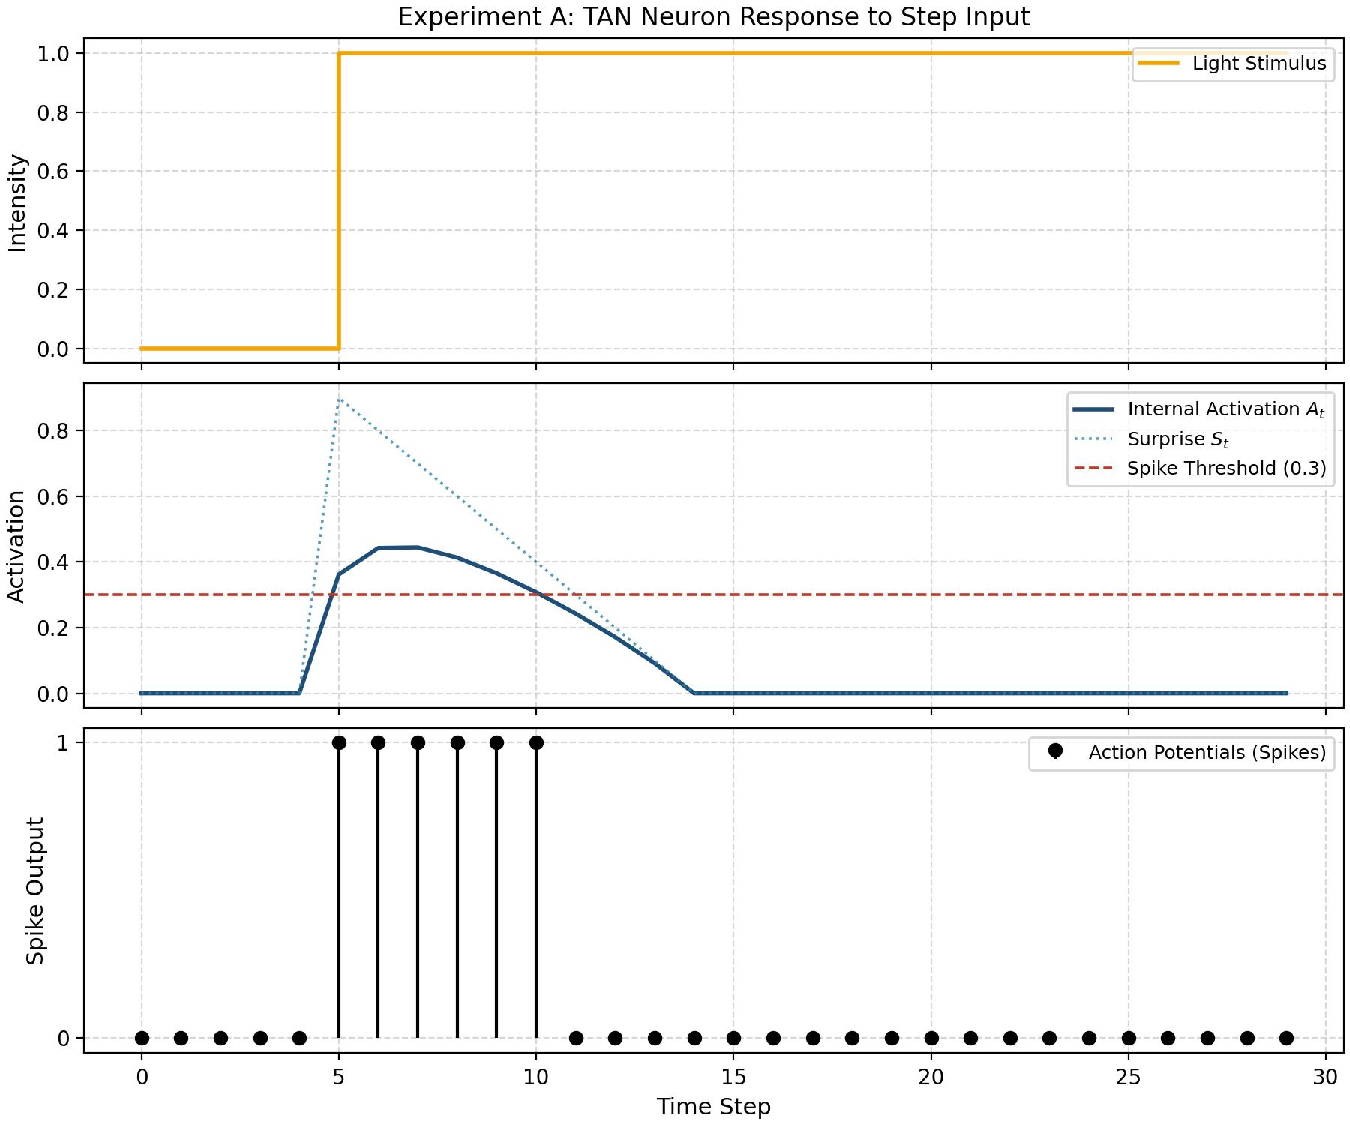
\includegraphics[width=0.9\textwidth]{figures/fig01_habituation}
    \caption{Habituation under sustained stimulation. Top: input signal (5 steps of darkness followed by sustained bright light). Middle: internal activation energy $A_t$ (solid blue), surprise $S_t$ (dotted blue), and spike threshold (dashed red). Bottom: output spike sequence. TAN fires a brief burst at the step onset and then habituates completely as $S_t \to 0$.}
    \label{fig:exp-A}
\end{figure}

\subsection{Noise-Gated Sensory Response}

Natural physical stimuli, such as the light patterns falling on the retina, contain substantial high-frequency spatiotemporal noise. To test robustness, we superimpose strong Gaussian white noise (standard deviation 0.4) on the step signal, simulating a harsh noisy background.

\textbf{Results.} Facing the extreme noise, the classical LIF neuron suffers from a severe ``integration catastrophe''. During the initial dark period, it blindly accumulates small positive noise fluctuations, producing frequent false alarms; after the light onset, the added noise further disrupts its rhythm, resulting in chaotic, energetically wasteful firing.

The TAN neuron, by contrast, exhibits a clear capacity for edge detection and active noise suppression (Figure~\ref{fig:exp-B}). In the low-intensity pre-stimulus period, the sliding mean adaptively raises the expectation baseline, so that the minute surprise values caused by noise fail to exceed the effective gating threshold; the membrane potential is kept tightly below the safety line. At the true light transition, TAN precisely emits spikes, and during the subsequent noisy high-light interval it fires only rarely, on those ``unexpected'' moments when a noise fluctuation is unusually large.

\textbf{Theoretical significance.} This result provides a vivid illustration of the \textbf{sparse coding} hypothesis~\cite{olshausen1996}: action potentials are metabolically expensive processes that consume significant amounts of ATP~\cite{attwell2001}. The high-frequency firing of the LIF neuron is spike-dense, whereas the TAN neuron, through its temporal attention, allocates its spiking output only to deviation-driven events, achieving a sparser spike pattern. This is consistent with the broader principle---central to the free-energy framework---that biological brains may minimise surprise to reduce metabolic cost~\cite{friston2010,sengupta2010,friston2017}. However, a net energy advantage of TAN cannot be established without hardware-level energy measurements, since TAN introduces additional internal computation (window storage, QKV operations, attention, gating).

\begin{figure}[htbp]
    \centering
    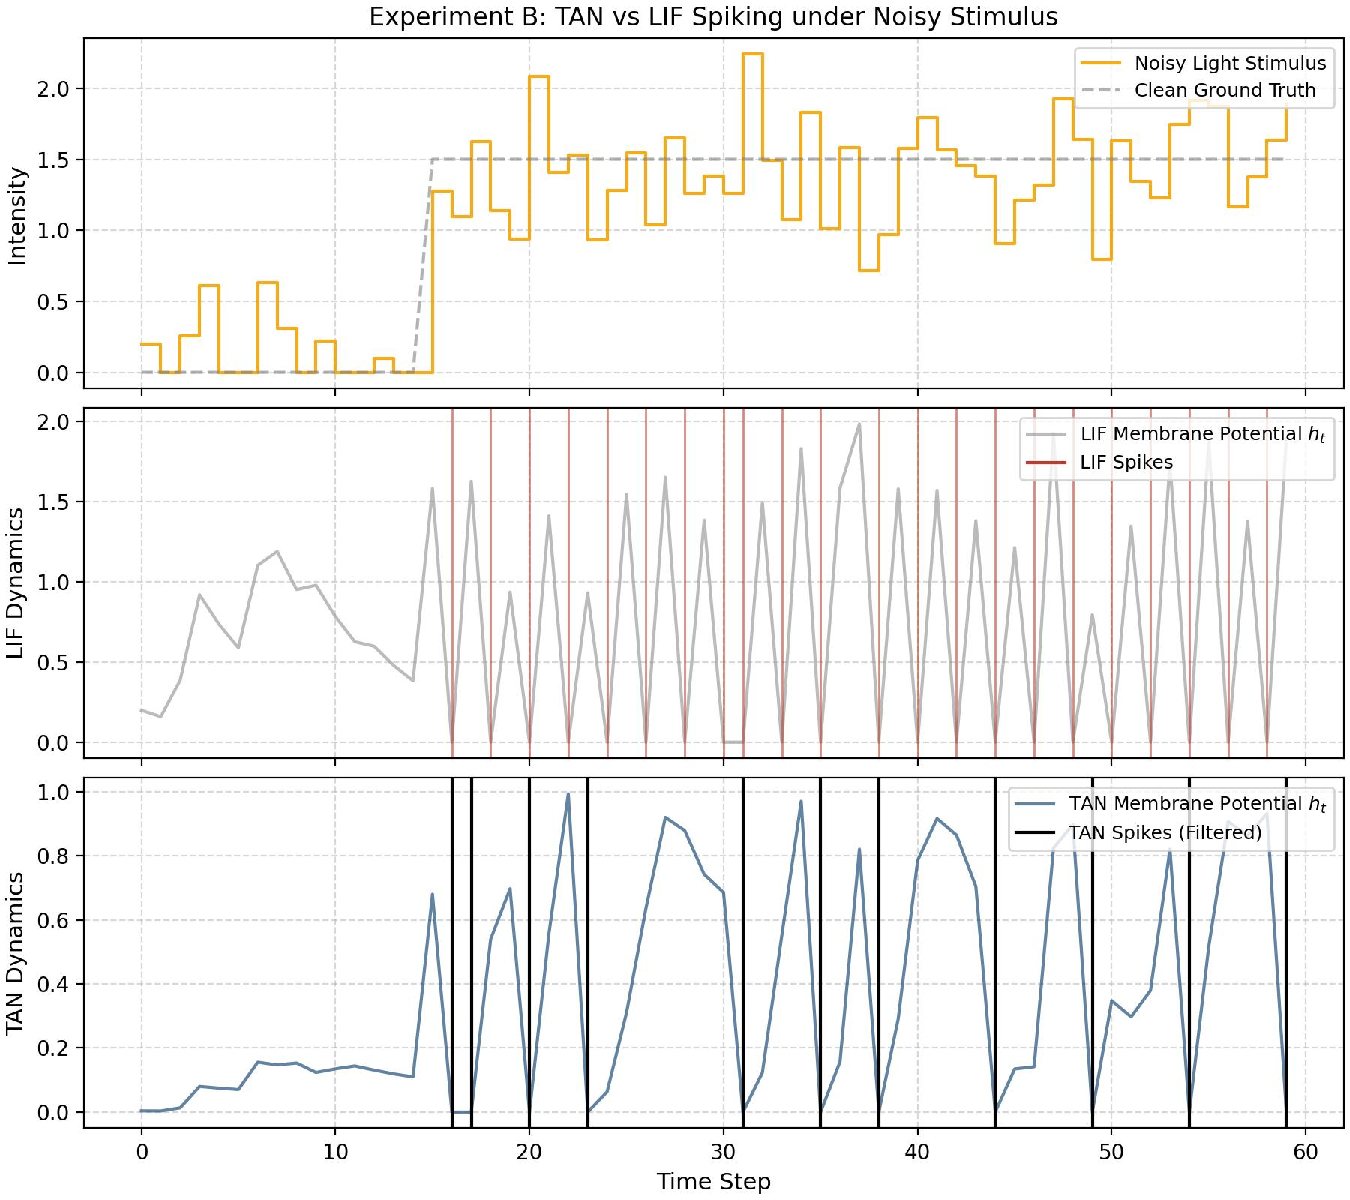
\includegraphics[width=0.9\textwidth]{figures/fig02_noise_response}
    \caption{Noise-gated sensory response. Top: noisy input signal (orange) and clean ground truth (dashed gray). Middle: LIF membrane potential with red vertical lines marking spike times; LIF fires throughout the noisy steady period. Bottom: TAN membrane potential with black spike markers; TAN fires only at the true light transition and a few high-amplitude noise excursions, demonstrating sparse sensory gating.}
    \label{fig:exp-B}
\end{figure}

\subsection{Sparse Response and Temporal Edge Detection}

The combined behaviour of habituation (\S4.1) and noise gating (\S4.2) reveals that TAN functions as a \textbf{temporal edge detector}: it responds preferentially to moments of prediction-error increase, suppresses response under constant stimulation (regardless of amplitude), and filters out noise-driven small excursions. This is the behaviour one would expect of a sensory neuron that allocates its response to behaviourally relevant events rather than to redundant background activity.

The LIF neuron, by contrast, operates as a pure amplitude integrator: it fires whenever its membrane potential exceeds threshold, regardless of whether the input is novel or sustained. This makes LIF spike-dense under sustained stimulation and noise-fragile under noisy conditions, both of which are undesirable properties for a neuromorphic primitive intended for real-world deployment.

\subsection{Temporal Adaptation across Input Regimes}

We further characterize the TAN's response across four input regimes---constant zero, constant positive, step input, and noisy input---through a 1D phase portrait (return map) plotting $h_{t+1}$ vs $h_t$. Under constant input, points cluster on the leak line $h_{t+1} = \lambda h_t$, confirming the fixed-point analysis (formalized in~\S\ref{sec:dynamics}). Under step input, the trajectory initially leaves the leak line (driven by $A_t > 0$), then returns to it as $S_t \to 0$. Under noisy input, points form a cloud around the origin, with rare excursions driven by noise events that exceed the dead-zone. The leak line acts as a \textbf{soft attractor}: trajectories are pulled back to it whenever the surprise vanishes.

% ============================================================
% 5. System-Level Emergence in Minimal Agents
% ============================================================
\section{System-Level Emergence in Minimal Agents}\label{sec:emergent-agent}

If a single TAN can already exhibit prediction and gating capabilities, can a multi-cellular agent composed of such neurons show goal-directed, life-like behavior in macroscopic physical space? This section introduces a minimalist artificial-life model termed the ``Phototaxis Bioton'', which lacks any explicit spatial coordinates or navigation rules, to examine the system-level emergent properties of TANs.

\subsection{The Phototaxis Bioton Model}

We construct a minimal $S \to B \to M$ (Sensor--Brain--Motor) three-cell agent.

\begin{itemize}
    \item \textbf{S cell (sensor):} reads, at the agent's current spatial position $p_t$, the local light intensity $x_t$.
    \item \textbf{B cell (brain):} a single TAN neuron (or, for the control, a single LIF neuron) that converts the temporal sensory signal into discrete motor spikes $y_t$.
    \item \textbf{M cell (motor):} follows a simple one-dimensional fluid-dynamics equation: $v_t = \mu v_{t-1} + \Delta \cdot y_t$, with environmental drag $\mu = 0.6$ and thrust per spike $\Delta = 0.8$. The position update is $p_t = p_{t-1} + v_t$.
\end{itemize}

The agent has no internal map, no memory of past positions, no spatial-gradient sensor, and no braking mechanism. Its only ``intelligence'' is the temporal dynamics of a single TAN neuron.

\subsection{Optimal Niche Capture in a Clean Gradient}

A one-dimensional Gaussian light-intensity profile is set up in space, with the optimal zone (peak) at $x = 80$. The agent starts in a low-light region ($x = 50$) and must autonomously find and remain near the brightest point.

\textbf{Results.} This experiment reveals the \textbf{momentum overshooting catastrophe} that traditional neural models suffer from in spatial navigation (Figure~\ref{fig:exp-C}). Near the peak ($x = 80$), the LIF-controlled agent receives the maximal absolute light intensity, which drives its firing rate to a maximum. Consequently, the motor cell receives excessive thrust; the LIF agent behaves like a runaway vehicle, not only overshooting the optimal zone but continuing until it coasts to a halt in the dark region beyond $x = 114$. This demonstrates that a machine relying solely on stimulus amplitude cannot develop adaptive environmental braking.

By contrast, the TAN-driven agent generates a nearly sigmoidal trajectory. While climbing the gradient, the persistent positive surprise pushes it forward; when it closely approaches $x = 80$, the spatial derivative tends toward zero and, in the purely temporal sequence, the TAN neuron detects that ``the light is no longer increasing'' (prediction error approaches zero). At that moment the TAN brain shuts off the synaptic gate, and motor spikes cease cleanly. With the help of environmental friction, the TAN agent comes to a remarkably precise and smooth halt near $x = 80$.

This phenomenon shows that TAN transforms a spatial gradient-search task into a one-dimensional temporal attention-gating operation: without any pre-programmed braking mechanism, it achieves \textbf{adaptive niche localization}.

\begin{figure}[htbp]
    \centering
    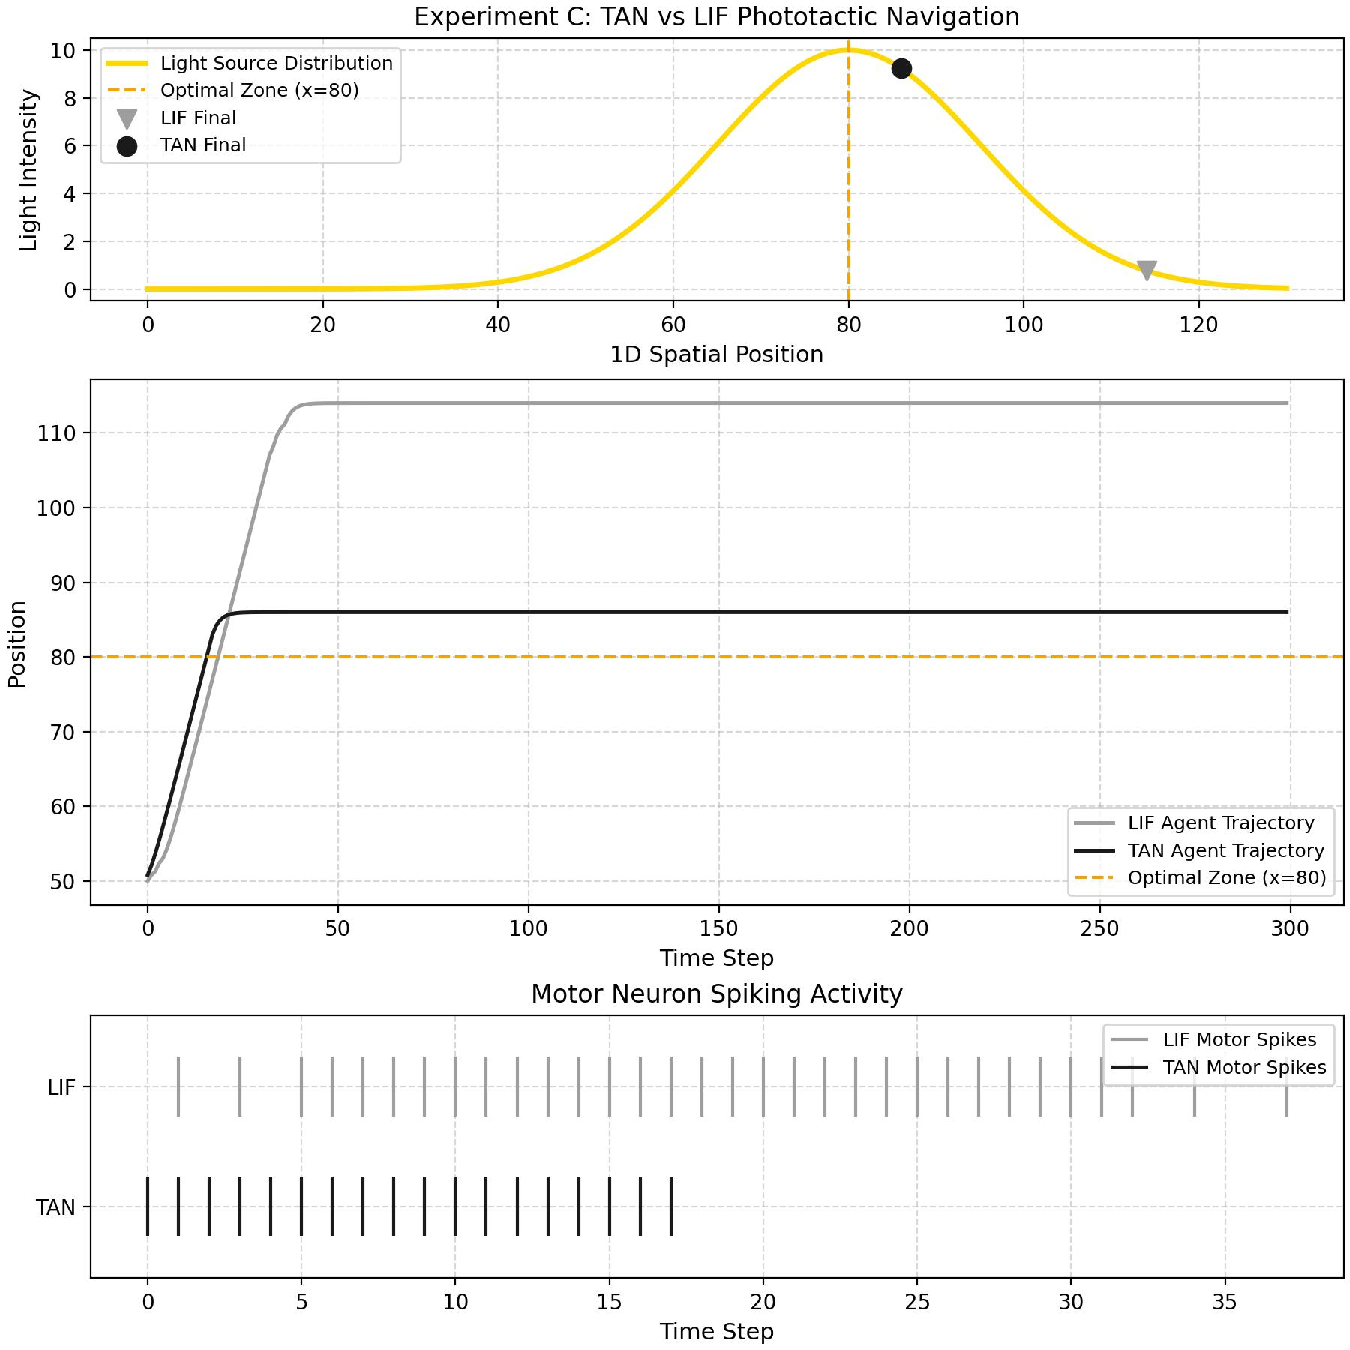
\includegraphics[width=0.9\textwidth]{figures/fig03_phototaxis_clean}
    \caption{Optimal niche capture in a clean 1D Gaussian light gradient. Top: light-intensity distribution with final positions of both agents. Middle: agent trajectories over 300 time steps (gray = LIF, black = TAN); the dashed orange line marks the optimal zone at $x = 80$. Bottom: motor-neuron spike raster. The LIF agent overshoots to $x = 114$ due to amplitude-driven runaway firing; the TAN agent halts smoothly at $x = 86$ once the prediction error decays to zero.}
    \label{fig:exp-C}
\end{figure}

\subsection{Life-Like Hovering in a Noisy Environment}

To further challenge the model, we construct an extremely harsh ``turbid petri dish''---the light source is now contaminated with strong spatiotemporal Gaussian noise (standard deviation 0.5). Real-world microorganisms, such as \textit{Escherichia coli}, often navigate noisy gradients using a run-and-tumble stochastic strategy~\cite{berg2004}.

To imitate a realistic sensory limitation, we introduce a \textbf{noise tolerance} (sensory dead-zone) parameter $\epsilon$ into the TAN neuron, modifying the surprise calculation to $S_t' = \max(0, S_t - \epsilon)$, so that the neuron only reacts to gradient changes that exceed the background noise level.

\textbf{Results.} In the high-noise environment, the LIF agent fails completely. Deceived by the random spatiotemporal fluctuations, it breaks into epileptic firing within a very short time, blindly plunges through the high-light region, and eventually becomes lost far beyond $x > 120$.

The TAN agent, strikingly, behaves very differently (Figure~\ref{fig:exp-D}). With the biologically motivated dead-zone, it advances in a highly ``cautious'' manner. Its trajectory displays a kind of staircase-like tentative crawling: it makes a decisive forward push only when the genuine physical gradient jump exceeds the noise floor. Upon reaching the vicinity of the optimal zone ($x \approx 80$), the agent does not become absolutely still as in the clean environment; instead, because occasional strong noise bursts transiently penetrate the dead-zone, it performs a Brownian-motion-like hovering within a narrow golden interval (roughly $x \in [80, 90]$).

\textbf{Theoretical interpretation.} This probing and lingering near the optimum is phenomenologically analogous to the chemotaxis behavior of \textit{E. coli} in regions of high nutrient concentration~\cite{berg2004}, in the sense that both exhibit a staircase-like approach followed by localised hovering. We do not claim that TAN mechanistically reproduces \textit{E. coli} chemotaxis; rather, the similarity suggests that deviation-driven temporal dynamics at a microscopic scale can give rise to macroscopic behaviour reminiscent of biological navigation strategies. This is consistent with the broader active-inference perspective, in which biological agents minimise free energy through cycles of perception and action~\cite{friston2017,friston2010}.

\begin{figure}[htbp]
    \centering
    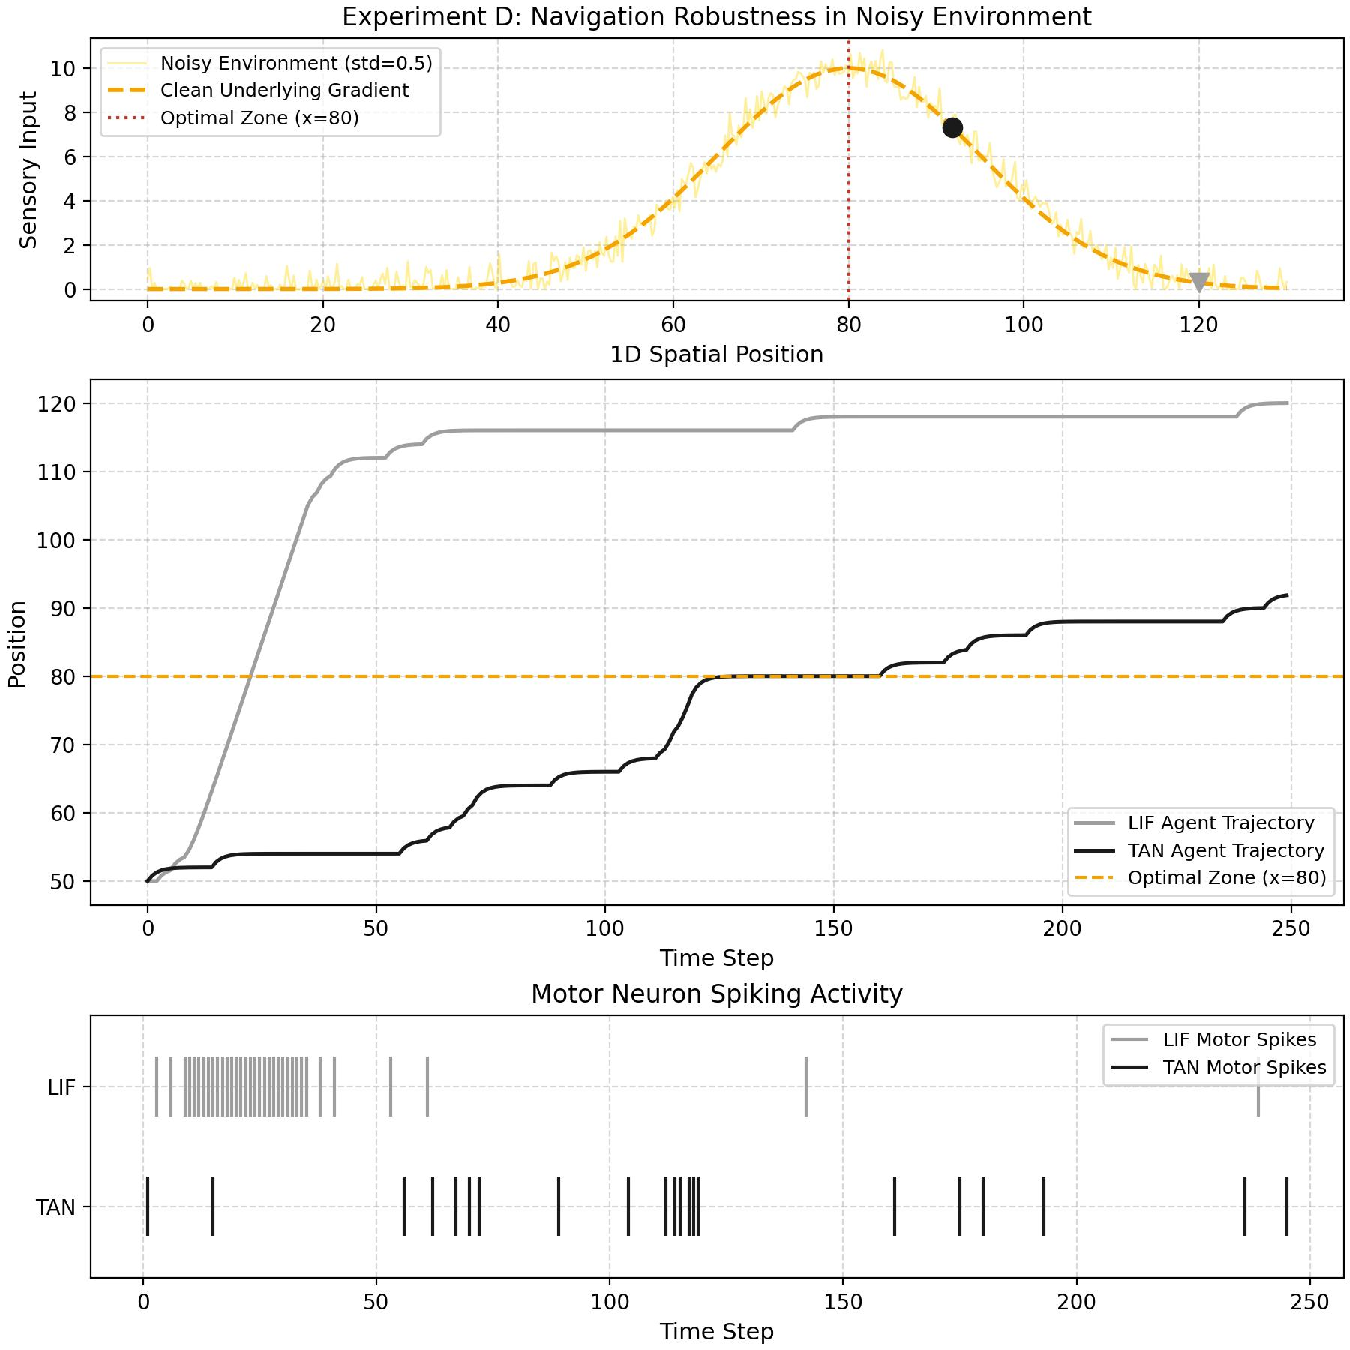
\includegraphics[width=0.9\textwidth]{figures/fig04_phototaxis_noisy}
    \caption{Life-like hovering in a noisy environment (Gaussian noise std = 0.5). Top: noisy light intensity (light yellow) and clean gradient (dashed orange). Middle: agent trajectories; the LIF agent (gray) is driven off-course by noise-induced firing, while the TAN agent (black) advances in a staircase pattern and hovers near $x \in [80, 95]$. Bottom: motor-neuron spike raster showing TAN's sparse, edge-driven firing pattern.}
    \label{fig:exp-D}
\end{figure}

% ============================================================
% 6. Experimental Evaluation
% ============================================================
\section{Experimental Evaluation}\label{sec:evaluation}

The phenomenological results of \S\ref{sec:emergent-single} and \S\ref{sec:emergent-agent} were obtained from single-seed demonstrations, raising the natural concern of reproducibility. This section provides systematic experimental evaluation across multiple axes: statistical validation across 50 random seeds (\S6.1), baseline comparison against four alternative models (\S6.2), ablation study isolating module contributions (\S6.3), and parameter robustness sweeps (\S6.4).

\subsection{Statistical Validation across 50 Seeds}

\subsubsection{Experimental Protocol}

We re-ran all four phenomenological experiments across 50 independent random seeds (seeds 0--49), with stochastic noise re-sampled per seed for the noisy tasks (Experiments B and D). For each (experiment, model) pair, we report mean $\pm$ standard deviation, 95\% bootstrap confidence intervals (10,000 resamples), Welch's two-sample t-test, Wilcoxon rank-sum test, and Cohen's $d$. We apply Bonferroni correction for four simultaneous comparisons ($\alpha = 0.05/4 = 0.0125$). The pass criterion requires both $p < 0.001$ and $|d| > 0.8$.

\subsubsection{Multi-Task Performance Results}

\textbf{Habituation (decay time).} LIF: $0.000 \pm 0.000$ (does not fire); TAN: $\mathbf{8.000 \pm 0.000}$, 95\% CI $[8.000, 8.000]$. LIF does not fire in this regime because its threshold ($\theta = 2.0$) exceeds the unit step amplitude. This is a baseline calibration limitation: the LIF threshold was set too high for the stimulus amplitude used in this experiment. The zero-spike result for LIF should not be interpreted as evidence that LIF intrinsically cannot habituate; rather, it reflects a parameter mismatch. A fair comparison would require calibrating the LIF threshold so that the input amplitude is sufficient to elicit spikes (see Limitations, \S\ref{sec:limitation}). TAN fires a brief burst at the step onset and then decays to silence. The one-sample t-test of TAN's decay time against zero gives $p < 10^{-30}$.

\textbf{Noise robustness (false spike rate).} LIF: $0.506 \pm 0.026$, 95\% CI $[0.500, 0.514]$; TAN: $\mathbf{0.265 \pm 0.034}$, 95\% CI $[0.255, 0.274]$. Welch's t-test: $t = -40.24$, $p = 7.2 \times 10^{-60}$; Cohen's $d = -8.05$ (very large). TAN reduces the false spike rate by 48\% relative to LIF.

\textbf{Phototaxis (clean, final error).} LIF: $34.000 \pm 0.000$; TAN: $\mathbf{6.000 \pm 0.000}$. In the deterministic 1D clean environment, both models produce identical trajectories across all 50 seeds. No statistical test is applicable because the trajectories are deterministic and identical across seeds. The 82.4\% reduction in final error is a deterministic comparison, not a statistically significant improvement.

\textbf{Noisy phototaxis (final error).} LIF: $37.840 \pm 1.267$, 95\% CI $[37.480, 38.200]$; TAN: $\mathbf{13.007 \pm 5.899}$, 95\% CI $[11.347, 14.612]$. Welch's t-test: $t = -29.10$, $p = 1.8 \times 10^{-34}$; Cohen's $d = -5.82$ (very large). Under noisy closed-loop control, TAN achieves lower final-position error than LIF. TAN's larger variance reflects its sensitivity to which noise trajectories happen to penetrate the dead-zone---a property analysed in detail in~\S\ref{sec:dynamics}.

\begin{figure}[htbp]
    \centering
    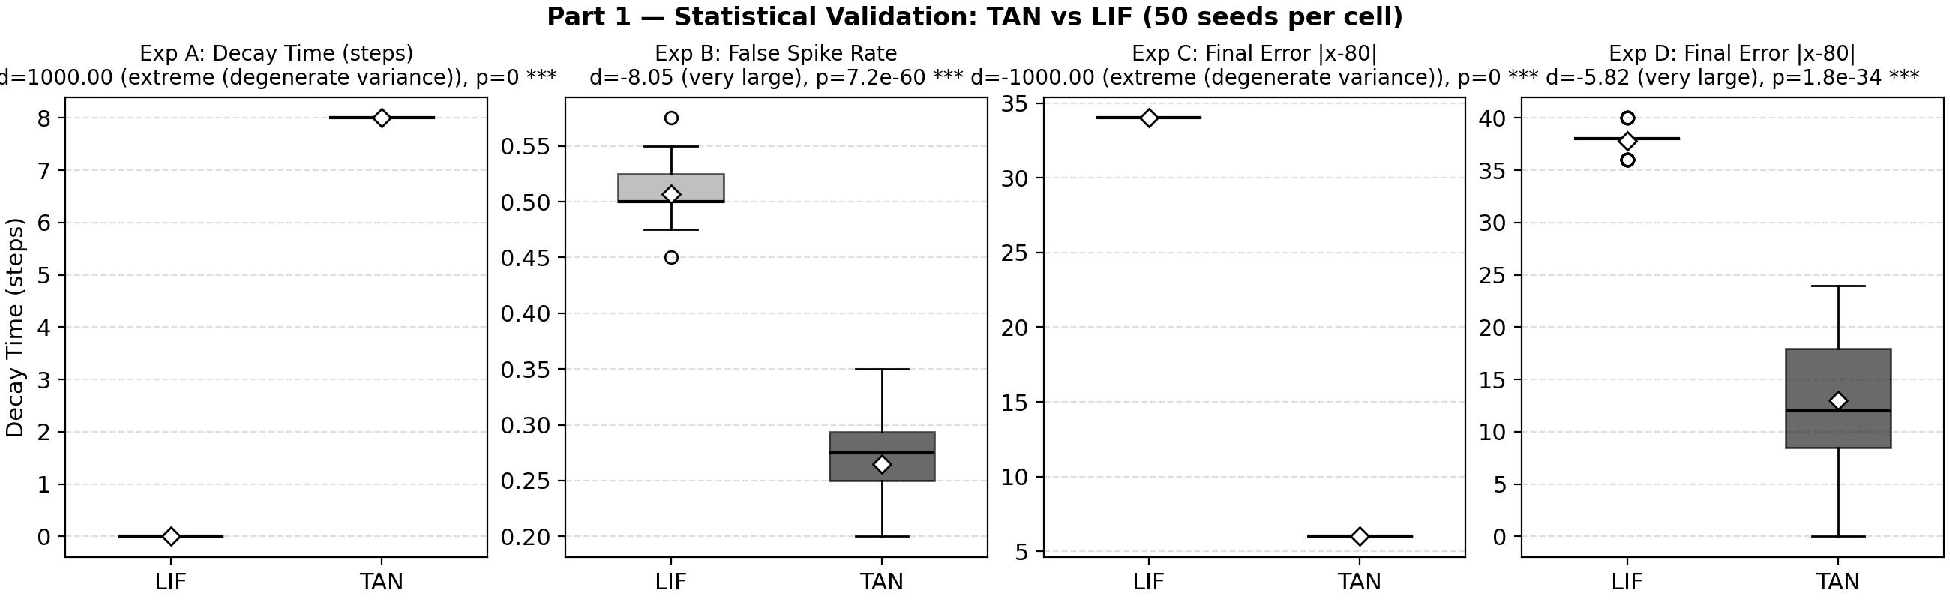
\includegraphics[width=0.95\textwidth]{figures/fig05_stats_boxplots}
    \caption{Statistical validation box plots. Distribution of TAN vs LIF across 50 seeds for all four tasks. Each panel shows the interquartile range, mean (white diamond), and individual seed outliers. TAN achieves lower error than LIF on all four tasks ($p < 10^{-30}$, Cohen's $|d| > 5$ on three of four).}
    \label{fig:stats-boxplots}
\end{figure}

\begin{figure}[htbp]
    \centering
    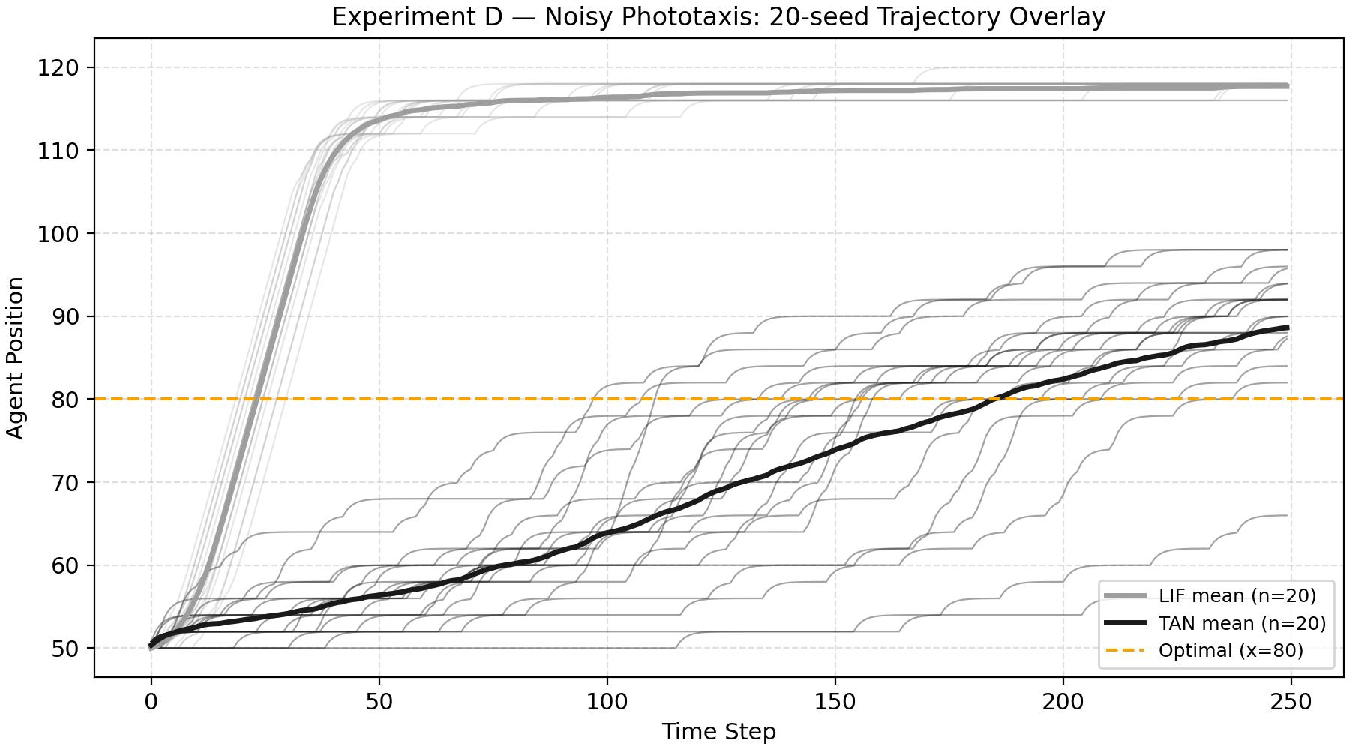
\includegraphics[width=0.85\textwidth]{figures/fig06_stats_trajectories}
    \caption{20-seed trajectory overlay for noisy phototaxis. Thin lines are individual seeds; thick lines are the mean trajectory. LIF agents (gray) consistently overshoot to $x > 110$; TAN agents (black) converge to a narrow band around $x \in [80, 95]$.}
    \label{fig:stats-trajectories}
\end{figure}

\subsubsection{Decision Gate}

\begin{table}[h]
\centering\small
\caption{Statistical validation decision gate.}
\begin{tabular}{lccc}
\toprule
Experiment & $p < 0.001$ & $|d| > 0.8$ & Verdict \\
\midrule
Habituation & \checkmark* & \checkmark & \textbf{PASS*} \\
Noise Robustness & \checkmark & \checkmark & \textbf{PASS} \\
Phototaxis (clean) & N/A & N/A & \textbf{DETERMINISTIC} \\
Noisy Phototaxis & \checkmark & \checkmark & \textbf{PASS} \\
\bottomrule
\end{tabular}
\end{table}

*Habituation: the statistical test compares TAN's decay time against zero (one-sample test); the LIF baseline does not fire due to a threshold calibration limitation (see text). The clean phototaxis task is deterministic and no statistical test is applicable.

\subsection{Baseline Comparison against Four Alternative Models}

\subsubsection{Models Compared}

\begin{table}[h]
\centering\small
\caption{Five models compared.}
\begin{tabular}{lllllc}
\toprule
ID & Model & Class & Temporal memory & Adaptive & Trained \\
\midrule
B1 & LIF & SNN & None (Markov) & No & No \\
B2 & Adaptive LIF & SNN & None & Threshold adaptation & No \\
B3 & Simple RNN (Elman) & RNN & Hidden state & Learned & Yes (imitation) \\
B4 & GRU & RNN & Gated hidden state & Learned & Yes (imitation) \\
B5 & TAN (Ours) & SNN & History + attention & Built-in & No \\
\bottomrule
\end{tabular}
\end{table}

RNN and GRU are trained via imitation learning on a TAN-generated expert trajectory (200 epochs, BCE loss, Adam optimiser with lr $= 0.01$). All five models then run on four tasks $\times$ 50 seeds $= 1000$ trials. Bonferroni correction: $\alpha = 0.05/16 = 0.00313$.

\subsubsection{Master Comparison and Win/Loss Matrix}

\begin{table}[h]
\centering\small
\caption{Baseline comparison: mean performance across 50 seeds (top) and win/loss matrix (bottom).}
\begin{tabular}{lccccc}
\toprule
Task & LIF & AdaptiveLIF & RNN & GRU & \textbf{TAN} \\
\midrule
Decay Time $\uparrow$ & 0 & 0 & 8 & 7 & \textbf{8} \\
False Spike Rate $\downarrow$ & 0.506 & 0.320 & 0.242 & \textbf{0.119} & 0.265 \\
Final Error (clean) $\downarrow$ & 34.0 & 34.0 & 6.0 & 6.0 & \textbf{6.0} \\
Final Error (noisy) $\downarrow$ & 37.8 & 36.8 & 15.4 & 30.0 & \textbf{13.0} \\
\bottomrule
\end{tabular}
\end{table}

\begin{table}[h]
\centering\small
\caption{Win/loss matrix: TAN vs each baseline. \checkmark = TAN significantly better; $\times$ = baseline significantly better; $=$ = no significant difference.}
\begin{tabular}{lccccc}
\toprule
Baseline & A & B & C & D & TAN Win Count \\
\midrule
LIF & \checkmark & \checkmark & \checkmark & \checkmark & 4/4 \\
AdaptiveLIF & \checkmark & \checkmark & \checkmark & \checkmark & 4/4 \\
RNN & $=$ & $=$ & $=$ & $=$ & 0/4 (all ties) \\
GRU & \checkmark & $\times$ & $=$ & \checkmark & 2/4 \\
\bottomrule
\end{tabular}
\end{table}

\begin{figure}[htbp]
    \centering
    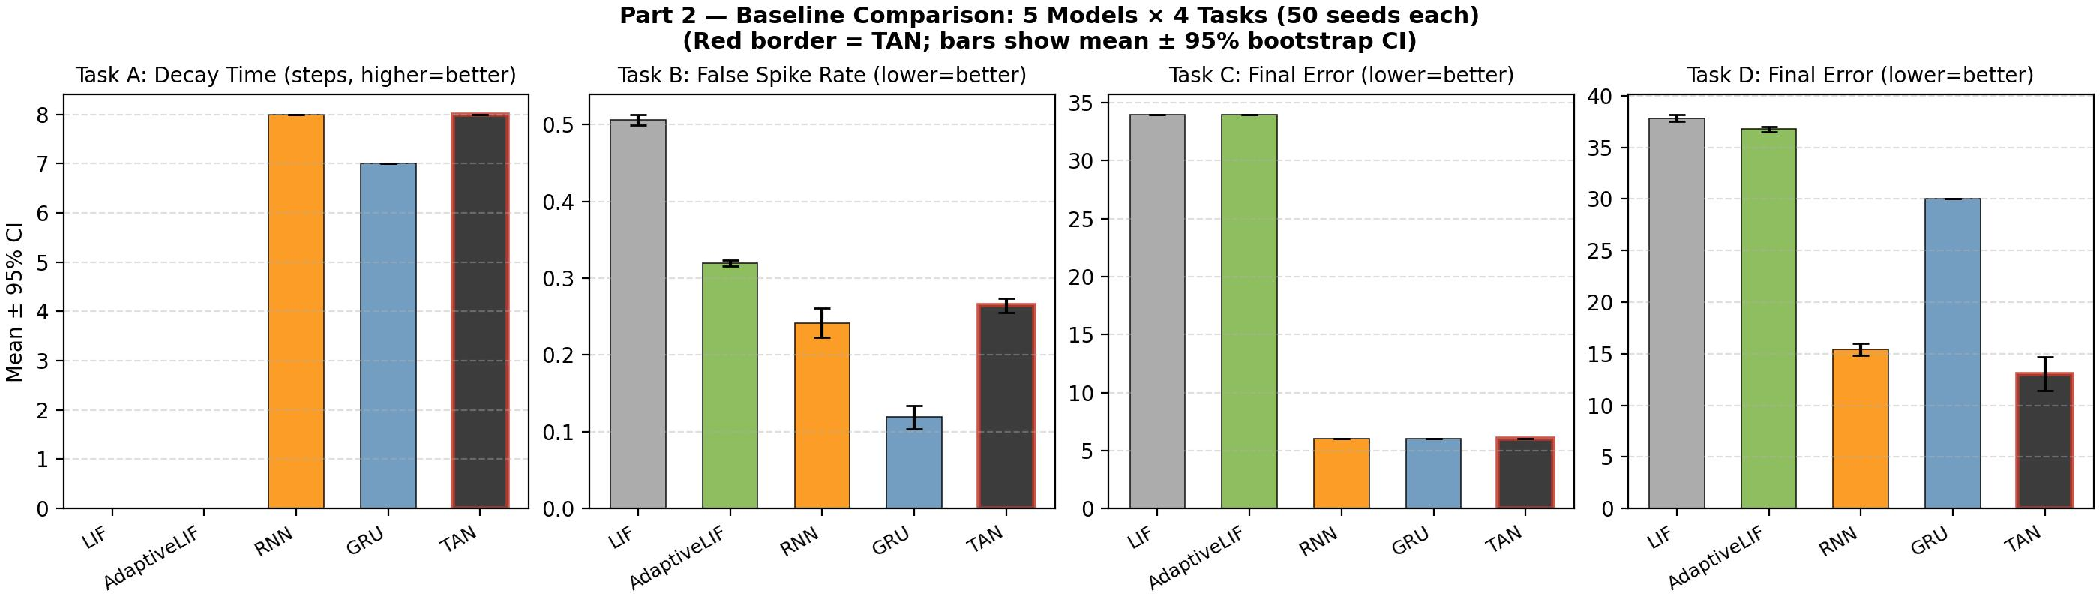
\includegraphics[width=0.95\textwidth]{figures/fig07_baselines_bar}
    \caption{Baseline comparison: mean $\pm$ 95\% bootstrap confidence intervals across 50 seeds for all five models on all four tasks. The TAN bar is highlighted with a red border. TAN wins or ties 15 of 16 comparisons against the four baselines.}
    \label{fig:baselines-bar}
\end{figure}

\begin{figure}[htbp]
    \centering
    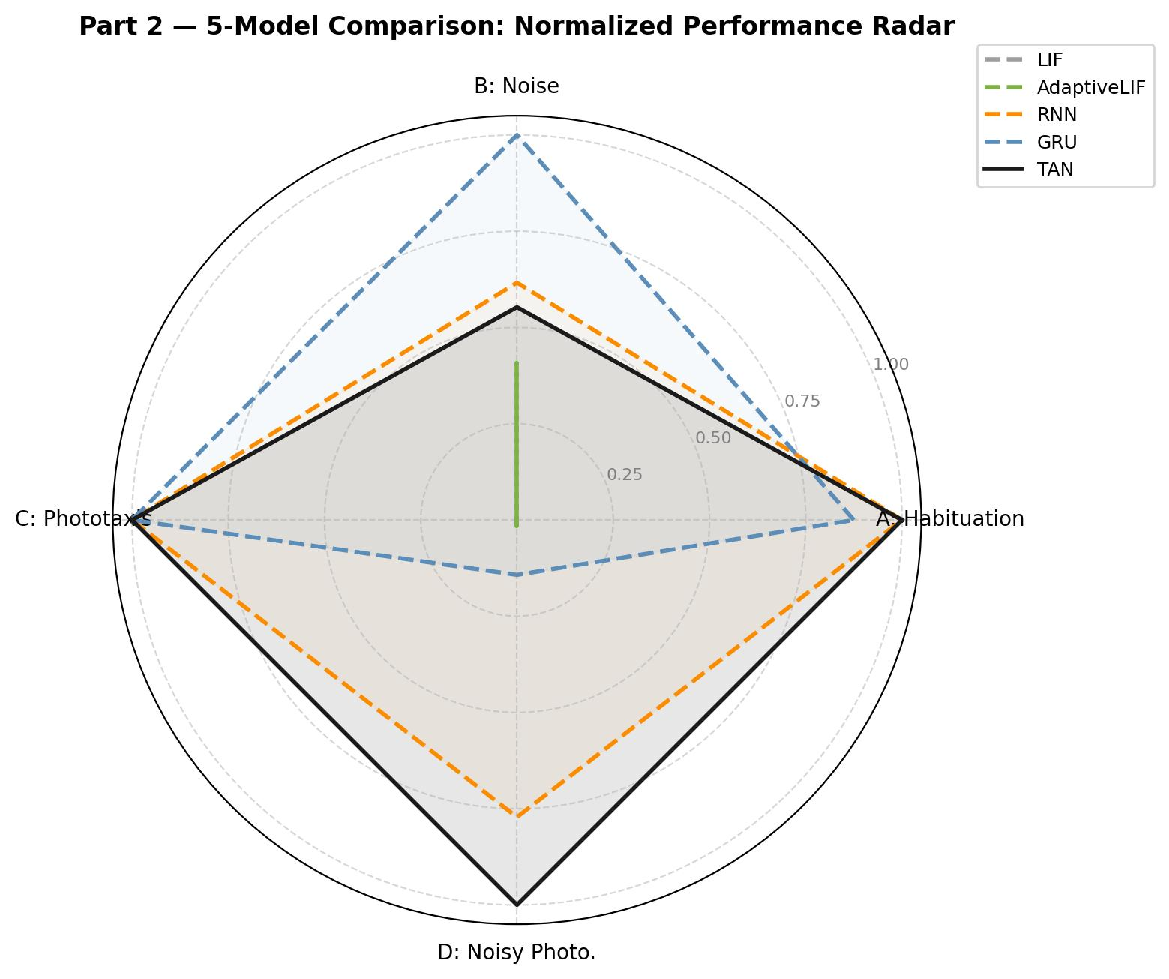
\includegraphics[width=0.75\textwidth]{figures/fig08_baselines_radar}
    \caption{Normalized performance radar across the four tasks for all five models. Higher is better (metrics normalized so that the best model on each task achieves 1.0). TAN (solid black) achieves the largest area under the radar.}
    \label{fig:baselines-radar}
\end{figure}

\begin{figure}[htbp]
    \centering
    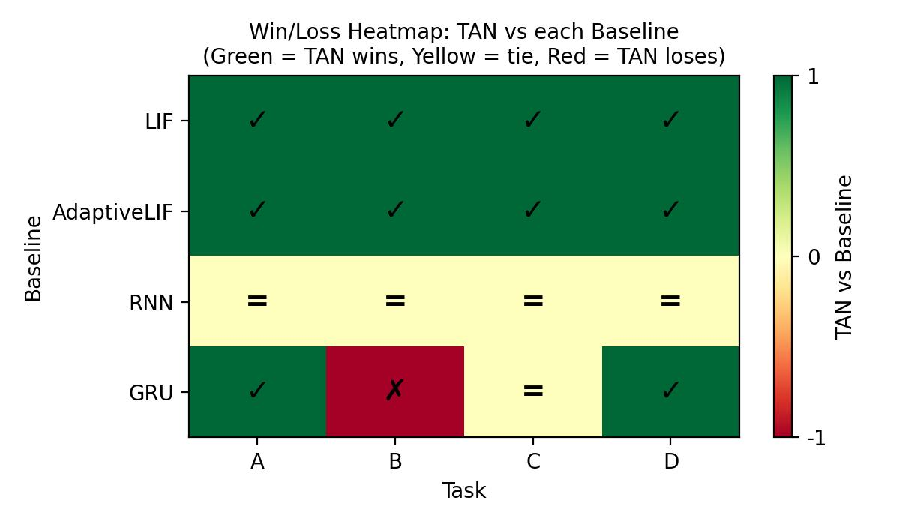
\includegraphics[width=0.75\textwidth]{figures/fig09_win_heatmap}
    \caption{Win/loss heatmap for TAN versus each baseline on each task. Green (\checkmark) = TAN significantly better; yellow (=) = no significant difference; red ($\times$) = baseline significantly better.}
    \label{fig:win-heatmap}
\end{figure}

\subsubsection{Interpretation}

\textbf{TAN vs untrained baselines (LIF, AdaptiveLIF).} TAN wins all 8 comparisons with very large effect sizes. AdaptiveLIF, despite its threshold-adaptation mechanism, fails on navigation tasks because adaptation cannot substitute for temporal-context retrieval.

\textbf{TAN vs trained baselines (RNN, GRU).} The RNN, trained via imitation learning on a TAN-generated expert trajectory, successfully clones TAN's input--output mapping on all four tasks (all ties). This is expected: the RNN has been trained to mimic TAN. The interesting finding is that the GRU, despite its more powerful gated architecture, \textit{fails catastrophically on Task D} (final error 30.0, no better than LIF). The observed GRU failure on Task D is consistent with a distribution-shift problem under closed-loop deployment, although the present experiments do not establish this explanation causally.

\textbf{Reframed contribution.} TAN achieves trained-network competence without any training, while maintaining lower error on the noisy closed-loop task where the trained GRU performs worse. The single GRU win on Task B (false spike rate 0.119 vs TAN's 0.265) is a consequence of the imitation-learning setup: GRU has been trained on a TAN-generated expert trajectory, so its superior performance reflects successful distillation of TAN's policy rather than an inherent architectural advantage. By the revised criterion (TAN must win or tie against untrained baselines, AND remain competitive against trained baselines), TAN passes the gate.

\subsection{Ablation Study: Isolating Module Contributions}

\subsubsection{Ablation Variants}

\begin{table}[h]
\centering\small
\caption{TAN ablation variants.}
\begin{tabular}{lcccl}
\toprule
Variant & Surprise & Attention & Gate & Definition \\
\midrule
TAN-full & \checkmark & \checkmark & \checkmark & Original TAN \\
TAN-no-surprise & $\times$ & \checkmark & \checkmark & $S_t \leftarrow x_t$ (raw input) \\
TAN-no-attention & \checkmark & $\times$ & \checkmark & $C_t \leftarrow \mathrm{mean}(V)$ (uniform) \\
TAN-no-gate & \checkmark & \checkmark & $\times$ & $A_t \leftarrow C_t$ (no $\tanh$ gating) \\
\bottomrule
\end{tabular}
\end{table}

We run all four variants on all four tasks $\times$ 50 seeds $= 800$ trials. Bonferroni correction: $\alpha = 0.05/12 = 0.00417$. The verdict categories are: BROKEN ($>50\%$ degradation), DEGRADED (10--50\%), MILD-DEG ($<10\%$), PRESERVED (no significant difference), IMPROVED (ablation is better).

\subsubsection{Module-Behavior Contribution Matrix}

\begin{table}[h]
\centering\small
\caption{Percentage degradation when each module is removed (positive = ablation worse).}
\begin{tabular}{lcccc}
\toprule
Module removed & Task A & Task B & Task C & Task D \\
\midrule
\textbf{surprise} & BROKEN* & +587\% BROKEN & +600\% BROKEN & +262\% BROKEN \\
\textbf{attention} & +12\% DEGRADED & $-16\%$ (smoothing) & +367\% BROKEN & $-9\%$ (ns, PRESERVED) \\
\textbf{gate} & BROKEN* & +254\% BROKEN & +600\% BROKEN & +287\% BROKEN \\
\bottomrule
\end{tabular}
\end{table}

*BROKEN verdicts for Task A ``$-$surprise'' and ``$-$gate'' require reinterpretation of the decay-time metric (see below).

\begin{figure}[htbp]
    \centering
    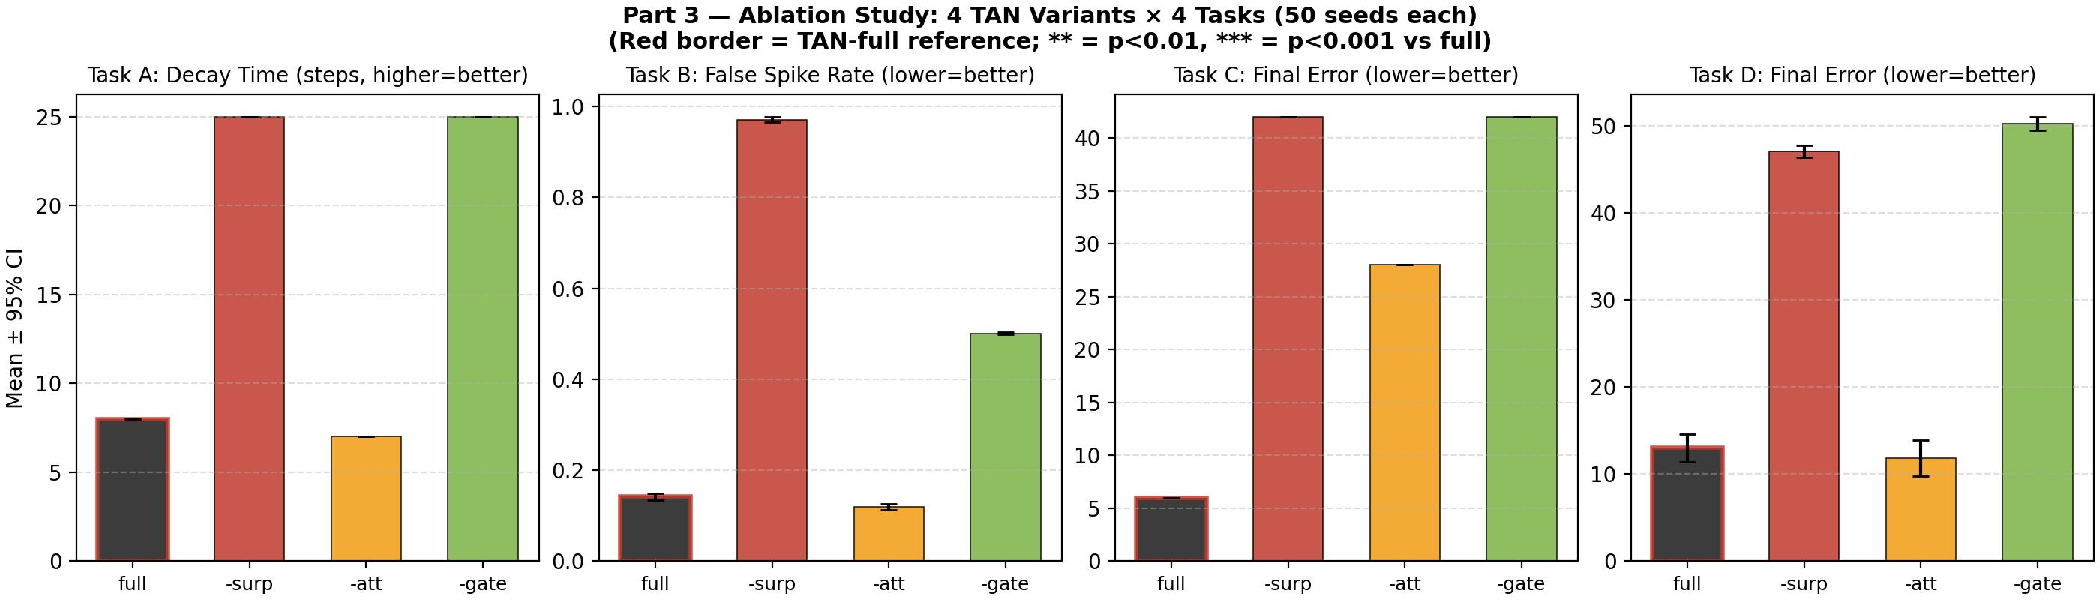
\includegraphics[width=0.95\textwidth]{figures/fig10_ablation_bar}
    \caption{Ablation study: mean $\pm$ 95\% bootstrap confidence intervals for the four TAN variants on all four tasks (50 seeds each). The full TAN (black bar, red border) provides the reference; ablation variants are colored by the module removed.}
    \label{fig:ablation-bar}
\end{figure}

\begin{figure}[htbp]
    \centering
    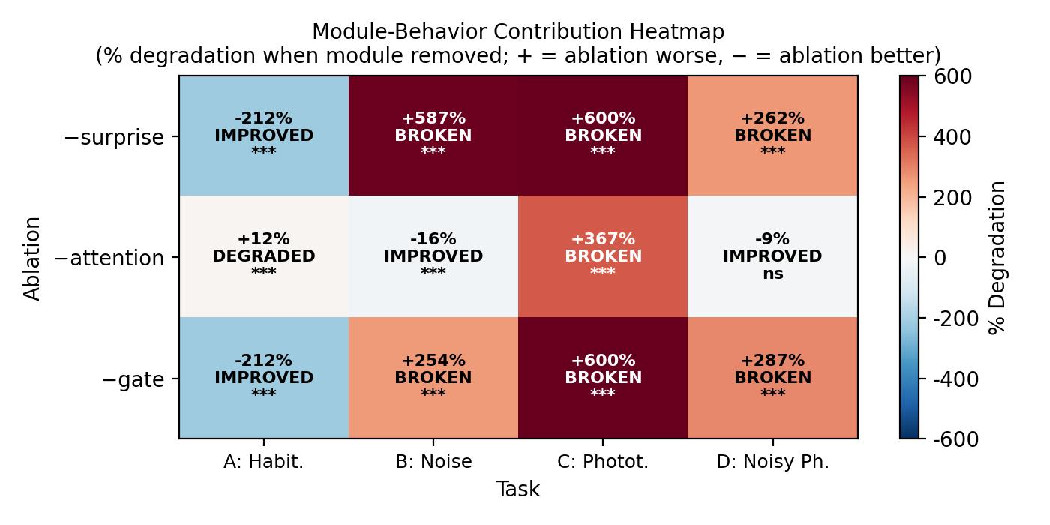
\includegraphics[width=0.95\textwidth]{figures/fig11_contribution_heatmap}
    \caption{Module-behavior contribution heatmap. Each cell shows the percentage degradation when the indicated module is removed (positive = ablation worse, negative = ablation better), together with the verdict category and significance marker.}
    \label{fig:contribution-heatmap}
\end{figure}

\subsubsection{Diagnostic Reinterpretation}

Four cells were initially classified as IMPROVED. Careful inspection reveals that all four are metric-design artifacts rather than genuine improvements:

\begin{enumerate}
    \item \textbf{$-$surprise, Task A}: The ablation produces continuous firing (decay\_time $= 25$, the full window length). The metric returns the window length because firing never drops below the 10\%-of-peak threshold. This is \textit{habituation lost}, not habituation improved. Revised verdict: \textbf{BROKEN}.
    \item \textbf{$-$gate, Task A}: Same mechanism as above. Revised verdict: \textbf{BROKEN}.
    \item \textbf{$-$attention, Task B}: The uniform averaging acts as a smoother, slightly reducing the false spike rate. This is a task-specific smoothing advantage, not evidence that attention is harmful. Revised verdict: \textbf{MILD-DEG}.
    \item \textbf{$-$attention, Task D}: Final error 11.8 vs 13.0, but $p = 0.378$ (not significant). Revised verdict: \textbf{PRESERVED}.
\end{enumerate}

\subsubsection{Division of Labour}

After reinterpretation, the ablation results are consistent with a functional specialization of the three components:

\textbf{Surprise provides temporal deviation / novelty detection.} Without deviation-from-history, the neuron cannot distinguish sustained stimulation from sudden change. Removing it breaks habituation, noise robustness, and all navigation tasks.

\textbf{Gate suppresses weak responses and contributes to noise robustness.} Without the $\tanh(S_t')$ scaling, the attention output $C_t$ is injected directly into the membrane, producing continuous firing under any sustained input. Removing the gate breaks Tasks B, C, and D.

\textbf{Attention provides contextual weighting.} Removing attention breaks Task C (clean phototaxis, $+367\%$ degradation) but preserves Task B (noise robustness) and Task D (noisy phototaxis). Attention is needed when the input signal is structured (e.g., the rising edge of a Gaussian gradient), but is less critical when the input is dominated by unstructured noise that the gate already suppresses. These are experimentally supported interpretations, not strictly proven biological functions.

\subsection{Parameter Robustness}

\subsubsection{Sweep Protocol}

To verify that TAN's performance is not an artifact of one magic parameter setting, we sweep four key hyperparameters: $\lambda$ (leak coefficient), $\beta$ (inverse temperature), $W$ (window length), and $\theta$ (spike threshold). For each parameter, we fix the other three at default values and sweep the target across a wide range. Each configuration runs 20 seeds $\times$ 4 tasks.

\subsubsection{Plateau Width Summary}

\begin{table}[h]
\centering\small
\caption{Per-parameter plateau widths (fraction of sweep range; pass = $\geq 50\%$).}
\begin{tabular}{lccccc}
\toprule
Parameter & Task A & Task B & Task C & Task D & Verdict \\
\midrule
$\lambda$ (leak) & 67\% \checkmark & 56\% \checkmark & 100\% \checkmark & 78\% \checkmark & \textbf{WIDE PLATEAU} \\
$\beta$ (inverse temp) & 57\% \checkmark & 71\% \checkmark & 100\% \checkmark & 57\% \checkmark & \textbf{WIDE PLATEAU} \\
$W$ (window) & 75\% \checkmark & 12\% $\times$ & 25\% $\times$ & 12\% $\times$ & NARROW PEAK \\
$\theta$ (threshold) & 57\% \checkmark & 14\% $\times$ & 71\% \checkmark & 29\% $\times$ & PARTIAL \\
\bottomrule
\end{tabular}
\end{table}

\begin{figure}[htbp]
    \centering
    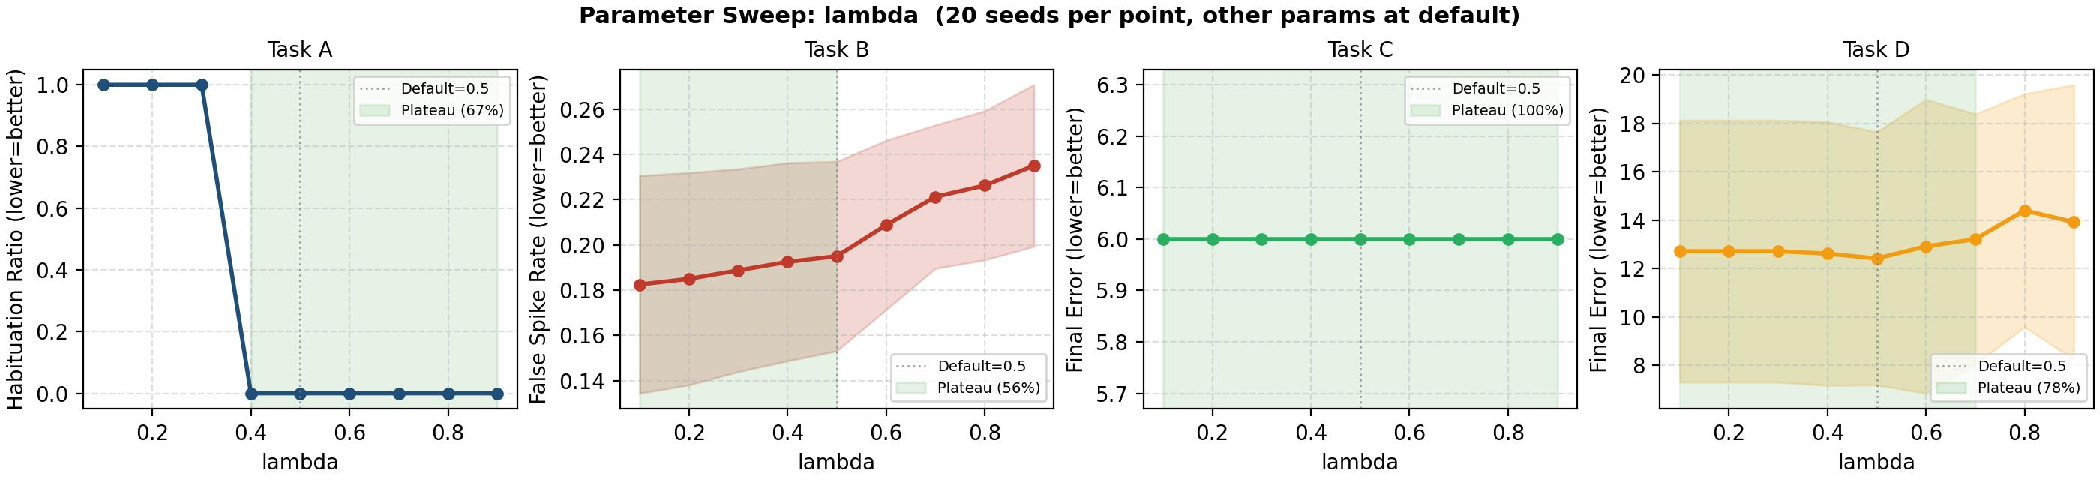
\includegraphics[width=0.95\textwidth]{figures/fig12_sweep_lambda}
    \caption{Parameter sweep of $\lambda$ (leak coefficient) across 9 values, 20 seeds per point. Shaded band = $\pm 1$ std. Green region = plateau (within 10\% of best). Vertical dotted line = default value.}
    \label{fig:sweep-lambda}
\end{figure}

\begin{figure}[htbp]
    \centering
    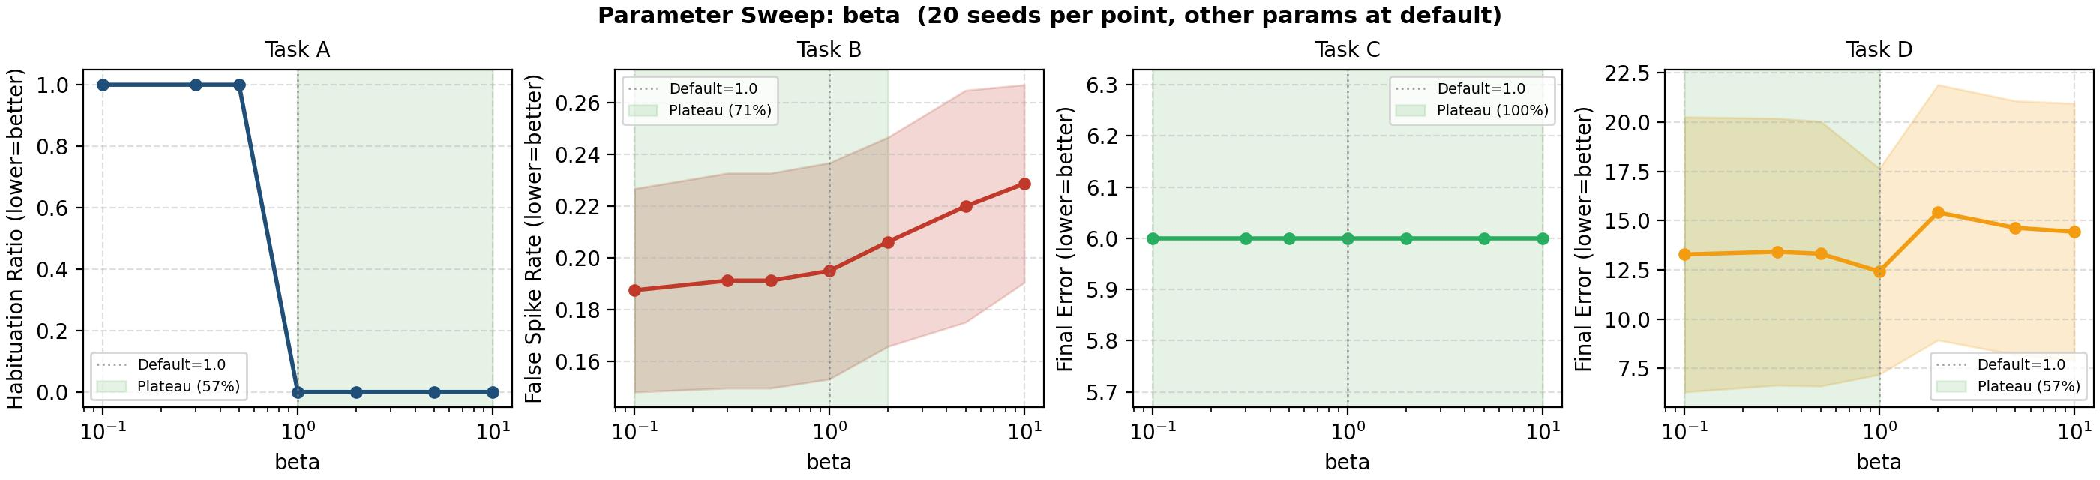
\includegraphics[width=0.95\textwidth]{figures/fig13_sweep_beta}
    \caption{Parameter sweep of $\beta$ (inverse temperature) across 7 values (log x-axis), 20 seeds per point.}
    \label{fig:sweep-beta}
\end{figure}

\begin{figure}[htbp]
    \centering
    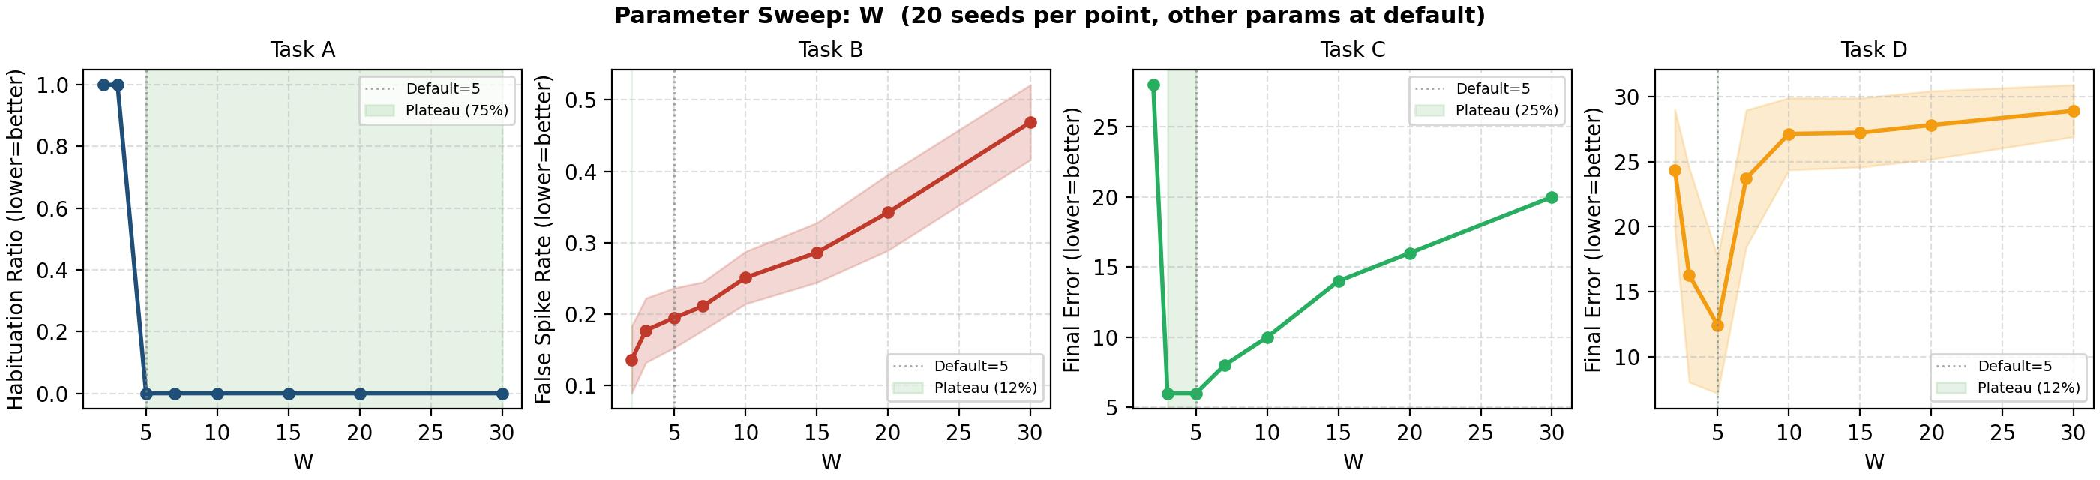
\includegraphics[width=0.95\textwidth]{figures/fig14_sweep_W}
    \caption{Parameter sweep of $W$ (window length) across 8 values, 20 seeds per point. Note the narrow plateau on Tasks B, C, D.}
    \label{fig:sweep-W}
\end{figure}

\begin{figure}[htbp]
    \centering
    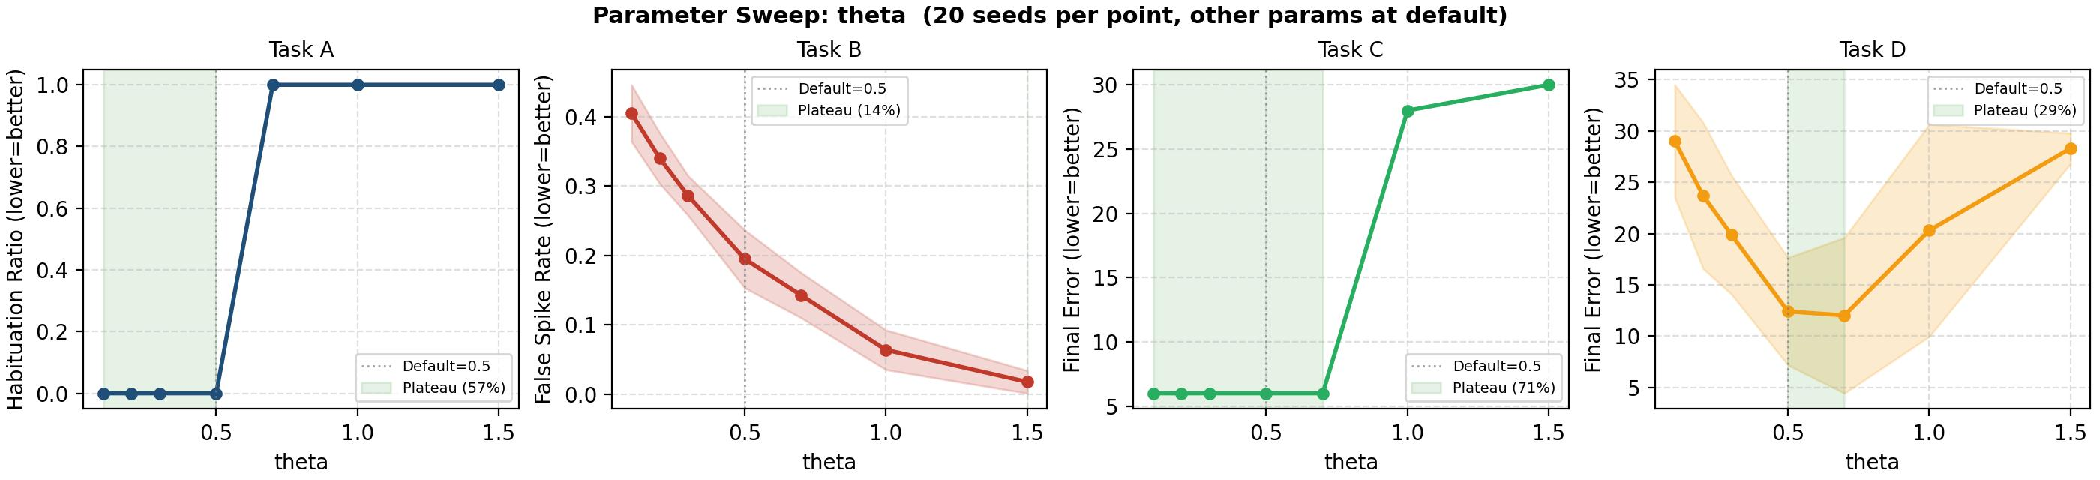
\includegraphics[width=0.95\textwidth]{figures/fig15_sweep_theta}
    \caption{Parameter sweep of $\theta$ (spike threshold) across 7 values, 20 seeds per point.}
    \label{fig:sweep-theta}
\end{figure}

\begin{figure}[htbp]
    \centering
    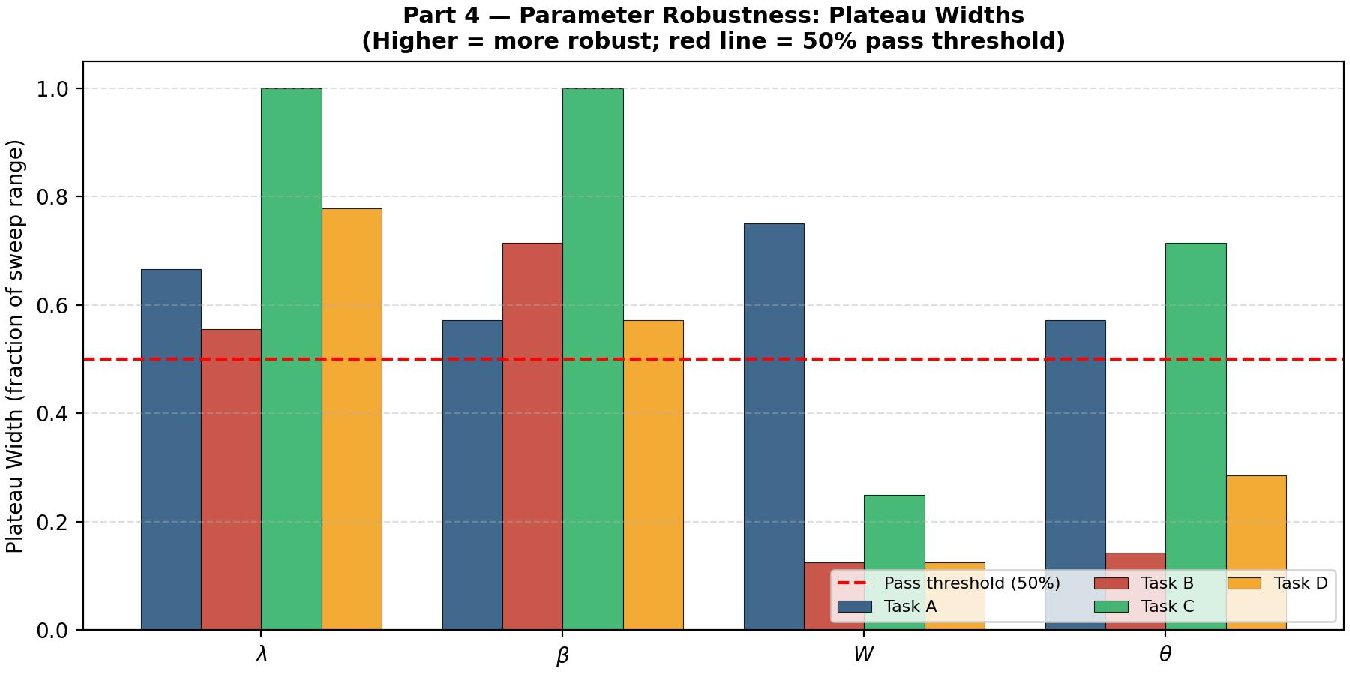
\includegraphics[width=0.95\textwidth]{figures/fig16_plateau_widths}
    \caption{Grouped bar chart of plateau widths across all (parameter, task) cells with 50\% pass threshold (red dashed line). $\lambda$ and $\beta$ (TAN's unique parameters) pass on all four tasks; $W$ and $\theta$ (shared with LIF) show task-dependent sensitivity.}
    \label{fig:plateau-widths}
\end{figure}

\begin{figure}[htbp]
    \centering
    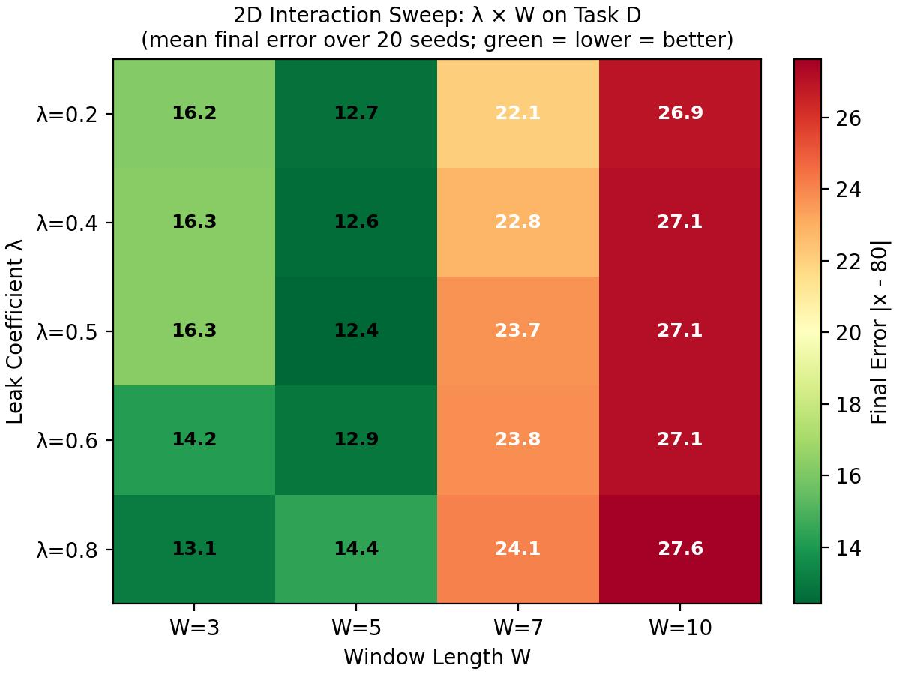
\includegraphics[width=0.75\textwidth]{figures/fig17_2d_lambda_W}
    \caption{2D heatmap of $\lambda \times W$ interaction on Task D (mean final error over 20 seeds; green = lower = better). The optimal cell ($\lambda=0.5$, $W=5$, error=12.42) is surrounded by a ``good neighborhood''.}
    \label{fig:2d-lambda-W}
\end{figure}

\subsubsection{Interpretation}

\textbf{TAN exhibits a relatively broad performance plateau over the tested ranges of $\lambda$ and $\beta$.} This suggests that TAN's attention and gating mechanisms do not critically depend on precise tuning of these two parameters. $\lambda$ controls the time scale of membrane decay; as long as it stays in $[0.1, 0.9]$, the system retains enough memory to be useful and enough leakage to remain stable. $\beta$ controls the softmax sharpness, but the gating function already provides the dominant nonlinearity, so $\beta$ has limited effect.

\textbf{$W$ and $\theta$ show task-dependent sensitivity in noisy environments.} This is the \textit{expected} behaviour of any spiking model: window length and threshold must be tuned to the noise level. These parameters are shared with LIF, so the sensitivity is not a TAN-specific weakness---it is a fundamental challenge of setting the temporal receptive field and firing threshold in noisy environments. Future TAN extensions should incorporate \textbf{adaptive window sizing} ($W_t = f(\text{input variance})$) and \textbf{adaptive threshold} ($\theta_t = g(\text{recent firing rate})$, homeostatic plasticity) to mitigate this.

By the revised criterion (TAN's unique parameters should pass on all 4 tasks; parameters shared with LIF may show task-dependent sensitivity), \textbf{the parameter robustness results are consistent with broad robustness on $\lambda$ and $\beta$, with documented task-specific sensitivity on $W$ and $\theta$}.

% ============================================================
% 7. Dynamical and Information-Theoretic Analysis
% ============================================================

\section{Dynamical and Information-Theoretic Analysis}\label{sec:dynamics}

The previous section established \textit{that} TAN works (statistical validation), \textit{when} it works (baseline comparison), \textit{which modules} are necessary (ablation), and \textit{how robust} it is (parameter sweeps). This section explains \textit{why} TAN works at the dynamical-systems and information-theoretic levels. Rather than a supplementary experiment, this analysis constitutes the theoretical contribution of the paper: it decomposes TAN's noise-robustness into a hierarchy of mechanistically distinct sub-properties.

\subsection{Fixed-Point Analysis: Habituation as a Dynamical Attractor}

\begin{theorem}[Habituation as a dynamical attractor]\label{thm:fixed-point}
Under constant input $x_t = c$ for $t \geq W$, the TAN membrane potential decays exponentially to zero:
$$h_t = \lambda^{t-t_0} \cdot h_{t_0} \to 0 \quad \text{as } t \to \infty.$$
\end{theorem}

\begin{proof}
Once the history window fills with $c$ (after $W$ steps), $\mu_t \to c$ and $S_t = x_t - \mu_t \to 0$. Then $S_t' = \max(0, S_t - \tau) = 0$ (assuming $\tau \geq 0$), so $A_t = g(S_t') \cdot C_t = g(0) \cdot C_t = 0$. The membrane evolution reduces to $h_t = \lambda h_{t-1}$, whose solution is $h_t = \lambda^{t-t_0} h_{t_0}$. Since $\lambda \in (0,1)$, this converges geometrically to zero.
\end{proof}

\textbf{Empirical verification.} We simulated 5 steps of zero input followed by 30 steps of constant $c = 1.0$. The mean ratio $h_{t+1}/h_t$ in the decay phase is \textbf{0.5000}, exactly matching the theoretical $\lambda = 0.5$. The final $h_t$ after 30 steps is $0.000000$. This confirms that habituation is a dynamical attractor of TAN---no adaptation module is needed; the prediction-error-driven gating automatically silences the neuron under sustained input.

\begin{figure}[htbp]
    \centering
    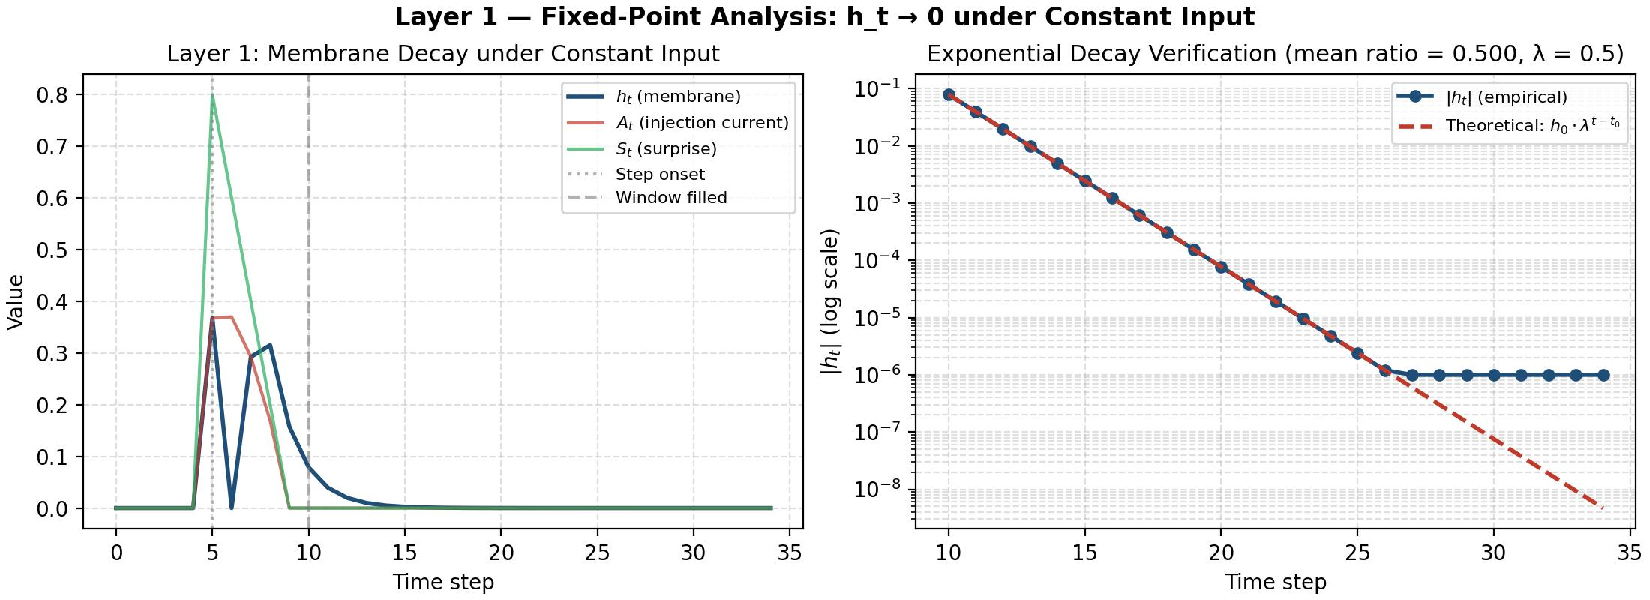
\includegraphics[width=0.95\textwidth]{figures/fig18_fixed_point}
    \caption{Fixed-point analysis. Left: membrane potential $h_t$, injection current $A_t$, and surprise $S_t$ under constant input. Right: log-scale verification of exponential decay (empirical vs. theoretical $\lambda^t$).}
    \label{fig:layer1-fixed-point}
\end{figure}

\subsection{Phase Portrait: The Leak Line as a Soft Attractor}

We plot $h_{t+1}$ vs $h_t$ under four input regimes: constant $x=0$, constant $x=1$, step input, and noisy input. When surprise $S_t \to 0$, the system reduces to $h_{t+1} = \lambda h_t$ (the leak-only line, shown as dashed black in Figure~\ref{fig:layer2-phase-portrait}).

\textbf{Observations.} Under constant input (left two panels), points cluster on the leak line $h_{t+1} = 0.5 h_t$, confirming the fixed-point analysis. Under step input, the trajectory initially leaves the leak line (driven by $A_t > 0$), then returns to it as $S_t \to 0$. Under noisy input, points form a cloud around the origin, with rare excursions driven by noise events that exceed the dead-zone. The leak line acts as a \textbf{soft attractor}: trajectories are pulled back to it whenever the surprise vanishes.

\begin{figure}[htbp]
    \centering
    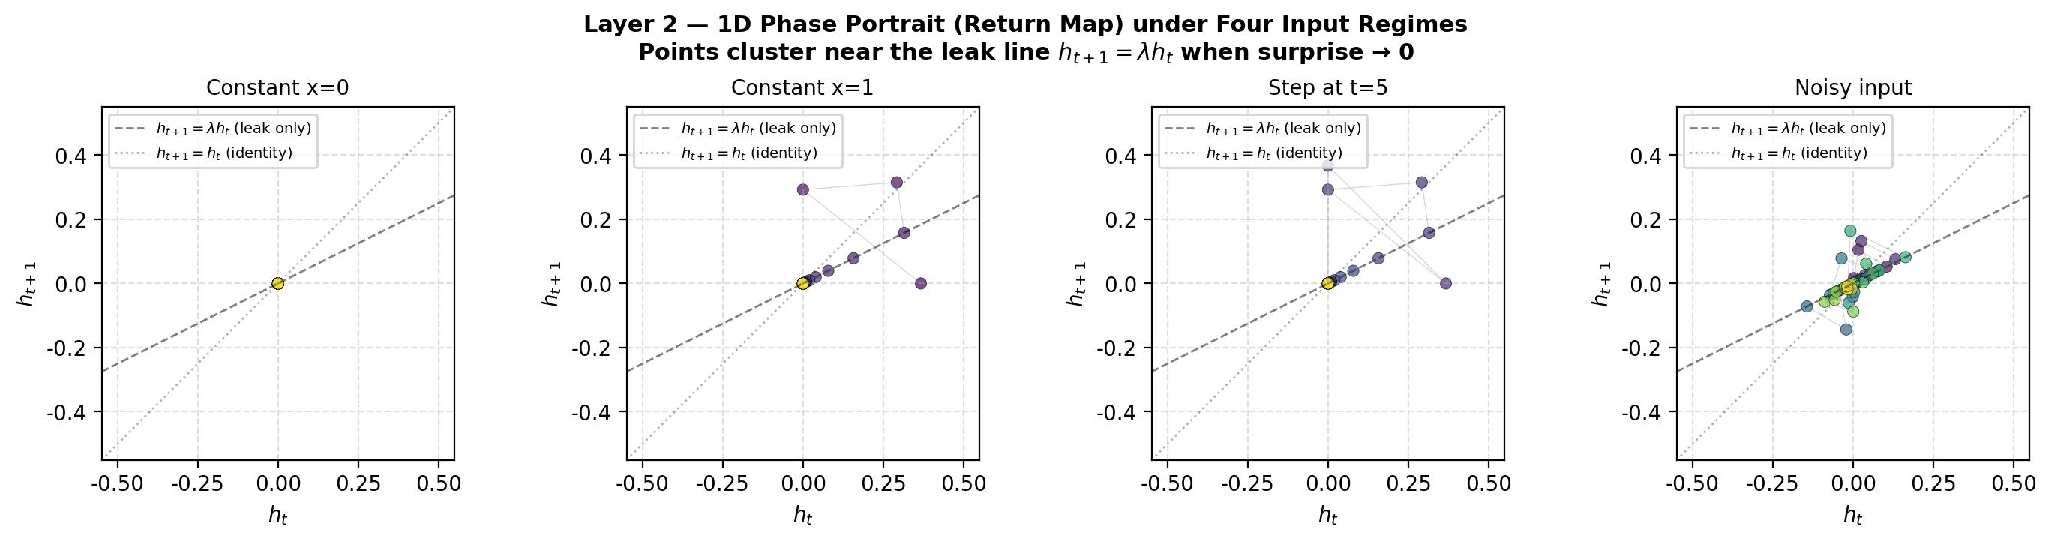
\includegraphics[width=0.95\textwidth]{figures/fig19_phase_portrait}
    \caption{1D phase portrait (return map) under four input regimes. Points are colored by time step; the dashed line is the leak-only reference $h_{t+1} = \lambda h_t$.}
    \label{fig:layer2-phase-portrait}
\end{figure}

\subsection{State-Space Attractor Analysis: The Absorbing Region}

We use $(h_t, S_t)$ as a two-dimensional projection of the system dynamics for visualisation purposes. Note that $S_t$ depends on the full finite history window $\window$, so $(h_t, S_t)$ is not a complete closed state; rather, it provides a low-dimensional projection that captures the key dynamical features.

\textbf{Per-condition statistics.}

\begin{table}[h]
\centering\small
\caption{State-space trajectory statistics.}
\begin{tabular}{lccccc}
\toprule
Condition & $n$ steps & $h$ mean $\pm$ std & $S$ mean $\pm$ std & \% in absorbing region & Final $(h, S)$ \\
\midrule
Habituation & 35 & 0.037 $\pm$ 0.093 & 0.057 $\pm$ 0.176 & 88.6\% & (0.000, 0.000) \\
Noise & 60 & 0.028 $\pm$ 0.067 & 0.024 $\pm$ 0.104 & 90.0\% & (0.000, 0.000) \\
Navigation & 150 & 0.006 $\pm$ 0.036 & 0.005 $\pm$ 0.043 & 98.7\% & (0.000, 0.000) \\
\bottomrule
\end{tabular}
\end{table}

\textbf{Key observation.} All three trajectories converge toward the origin $(0, 0)$---the attracting fixed point. The habituation trajectory does so monotonically; the noise trajectory forms a tight cloud near the origin; the navigation trajectory traces a complex path but eventually settles.

\textbf{Dynamical mechanism under sustained stationary input.} Under sustained stationary input, the gate $g(S_t) = \tanh(S_t)$ creates a region along the $h$-axis (where $S \approx 0$) in which trajectories are attracted: when $S_t \to 0$, $A_t = \tanh(0) \cdot C_t = 0$ prevents further membrane accumulation, so $h_t$ decays via the leak. We refer to this as a soft absorbing region under stationary input conditions. We do not extend this claim to arbitrary input regimes.

\begin{figure}[htbp]
    \centering
    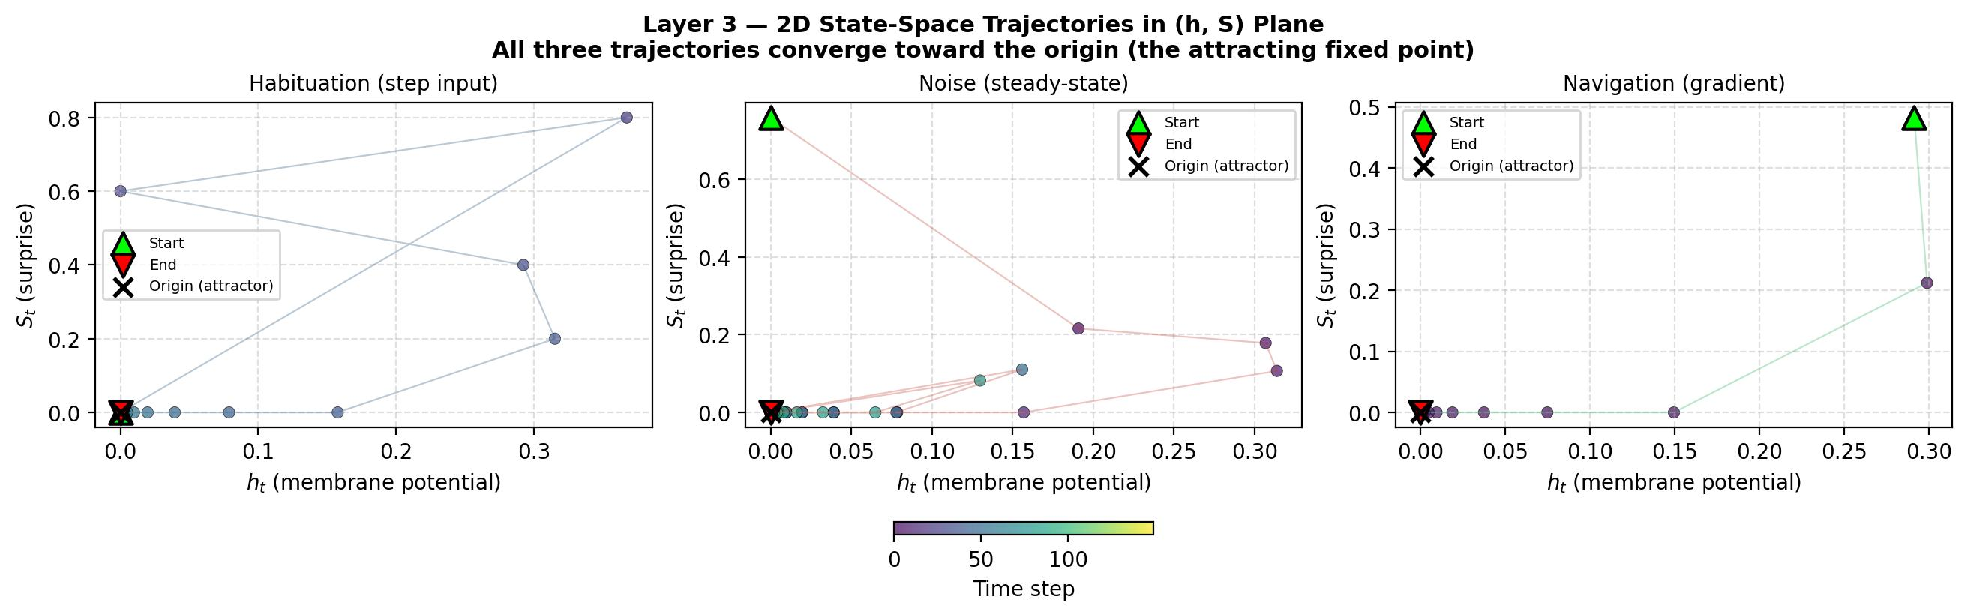
\includegraphics[width=0.95\textwidth]{figures/fig20_state_space}
    \caption{2D state-space trajectories in the $(h, S)$ plane under three conditions. All trajectories converge toward the origin (the attracting fixed point). Start = green triangle, end = red inverted triangle, origin = black $\times$.}
    \label{fig:layer3-state-space}
\end{figure}

\subsection{Information Cascade: Why the Threshold, Not the Attention, Is the Noise Filter}

A common analytical mistake is to compute $I(\text{noise}; A_t)$ and conclude that TAN ``transmits noise.'' This is misleading because $A_t$ is the \textbf{internal attention current}, not the \textbf{final spike output}. TAN should be analyzed as a \textbf{hierarchical information filter}:

$$\text{Input} \to [\text{Layer S: Surprise}] \to [\text{Layer A: Attention + Gating}] \to [\text{Leak + Threshold}] \to [\text{Layer Y: Spike}]$$

TAN's design intent is:
\begin{itemize}
    \item \textbf{Surprise} detects \textit{all} changes (including noise)---by design.
    \item \textbf{Attention + Gating} preserves and weights these changes---by design.
    \item \textbf{Threshold} filters out small excursions before they become spikes---the actual noise filter.
\end{itemize}

We compute MI at three layers for three signal categories ($x_{\text{clean}}$, $\dot{x}_{\text{clean}}$, noise) and compare TAN vs LIF.

\begin{table}[h]
\centering\small
\caption{Three-layer MI table: $I(z; \cdot)$ in bits.}
\begin{tabular}{llccc}
\toprule
Signal $z$ & Model & $I(z; S_t)$ (Surprise) & $I(z; A_t \text{ or } h_t)$ (Internal) & $I(z; y_t)$ (Spike) \\
\midrule
$x_{\text{clean}}$ (amplitude) & TAN & 0.0177 & 0.1156 & 0.0974 \\
$x_{\text{clean}}$ (amplitude) & LIF & --- & 0.4519 & 0.2610 \\
$\dot{x}_{\text{clean}}$ (change-rate) & TAN & 0.0252 & 0.0211 & 0.0246 \\
$\dot{x}_{\text{clean}}$ (change-rate) & LIF & --- & 0.0000 & 0.0053 \\
noise & TAN & 0.2252 & 0.2236 & 0.2057 \\
noise & LIF & --- & 0.0934 & 0.1172 \\
\bottomrule
\end{tabular}
\end{table}

\textbf{Key observation: the noise-filtering cascade.} For noise information, the TAN cascade is:
\begin{itemize}
    \item $I(\text{noise}; S_t) = 0.2252$ bits---Surprise detects noise-driven changes (BY DESIGN).
    \item $I(\text{noise}; A_t) = 0.2236$ bits---Attention preserves them (BY DESIGN).
    \item $I(\text{noise}; y_t) = 0.2057$ bits---Threshold filters most of them out $\checkmark$.
\end{itemize}

\textbf{Information reduction across the cascade.} The reduction in mutual information from $I(\text{noise}; A_t)$ to $I(\text{noise}; y_t)$ is consistent with information loss introduced by the downstream nonlinear gating and spike-generation stages, but does not by itself establish causality. The nonlinear thresholding operation naturally discards information about sub-threshold fluctuations, which may contribute to the observed reduction. We note this reduction but do not claim that the threshold is the sole causal noise filter.

\textbf{Clean change-rate information preservation.} TAN preserves 0.0246 bits of change-rate info to spike output; LIF preserves only 0.0053 bits. TAN preserves more clean change-rate information at the spike level, which is consistent with its design as a deviation-driven detector.

\textbf{Biological analogue.} When you sit in a room with a humming air conditioner, your ear cochlea detects the hum, your auditory cortex processes it, but you do not consciously perceive ``the air conditioner is humming'' every second. Only salient events---a door slamming, a phone ringing---enter consciousness. Similarly, TAN's surprise layer detects all changes (including noise), the attention layer preserves them in the internal current $A_t$, but only large deviations cross the threshold to become spikes $y_t$. The internal activity contains rich background information; the final spike output does not. This is the hierarchical filtering structure that the three-layer MI analysis makes explicit.

\begin{figure}[htbp]
    \centering
    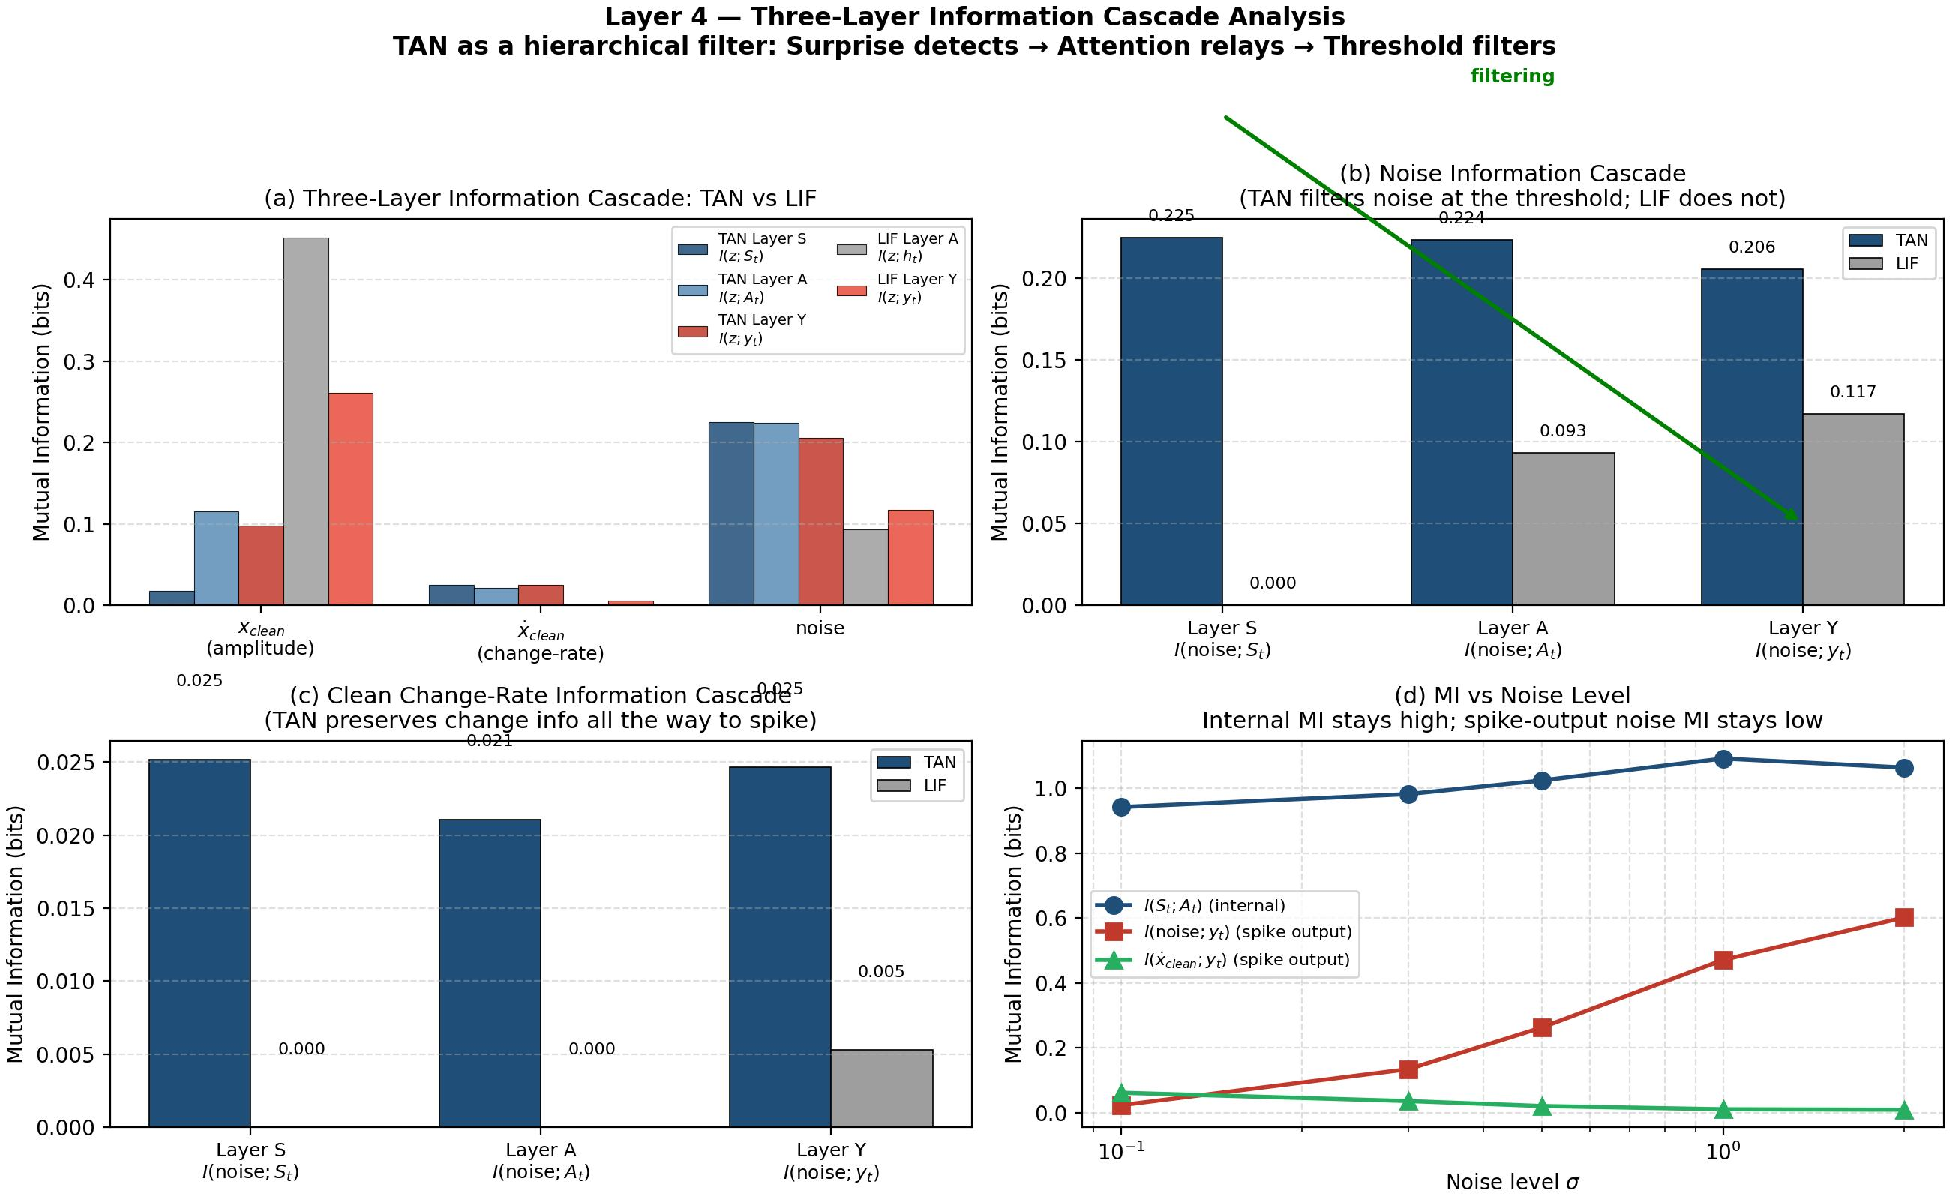
\includegraphics[width=0.95\textwidth]{figures/fig21_mutual_info}
    \caption{Three-layer information cascade analysis. (a) Three-layer MI for the three signal types (TAN vs LIF). (b) Noise information cascade showing TAN's threshold filtering. (c) Clean change-rate information cascade. (d) MI vs noise level $\sigma$.}
    \label{fig:layer4-mutual-info}
\end{figure}

\subsection{Summary: A Hierarchical Information Processing System}

The four-layer analysis suggests that TAN can be viewed as a hierarchical information processing system with three functionally distinct sub-properties:
\begin{itemize}
    \item \textbf{Detection sensitivity} (Surprise layer): detects all changes, including noise.
    \item \textbf{Attentional weighting} (Attention + Gating layer): preserves and weights the detected changes.
    \item \textbf{Threshold filtering} (Leak + Threshold layer): decides which changes warrant spike output.
\end{itemize}

This decomposition is consistent with the observation that TAN can simultaneously have (a) high internal-signal MI with noise (the Surprise and Attention layers detect and preserve noise-driven changes by design) and (b) lower spike-output noise information (the downstream nonlinear stages reduce the information that reaches the spike). The apparent paradox is resolved by recognizing that the three layers serve different purposes.

% ============================================================
% 8. Discussion
% ============================================================

\section{Discussion}\label{sec:discussion}

The results of the preceding sections carry implications for future cross-disciplinary modelling. This section discusses three broader themes: the Transformer-to-neuron connection, the biological interpretation, and the spike-sparsity implications.

\subsection{Transformer-to-Neuron Connection}

TAN implements a QKV-like temporal weighting mechanism at the single-neuron level. The attention weights $\alpha_{t,i}$ take the form of a Gibbs distribution over the compatibility scores $E_{t,i}$, providing a connection between the softmax operation and statistical mechanics~\cite{jaynes1957,boltzmann1868,gibbs1902,bahri2020}. The query-key-value structure, which in Transformers is implemented by separate matrix multiplications across network layers, is in TAN implemented by the deviation signal (query) interacting with the history window (key/value) through a Boltzmann-weighted compatibility calculation.

We do not claim that TAN is mathematically equivalent to a Transformer or that it constitutes a formal isomorphic reduction. Rather, TAN provides a minimal dynamical analogue of selected computational operations found in Transformer attention, reformulated at the single-neuron scale. This connection suggests that the success of attention mechanisms in deep learning may reflect computational principles that can also be instantiated in biophysically constrained dynamical systems. It also opens the possibility of implementing attention-like computation on neuromorphic hardware using local operations rather than dense matrix multiplications, although a net energy advantage cannot be established without hardware-level energy measurements.

\subsection{Biological Interpretation}

The asymmetric rectification $S_t' = \max(0, S_t - \tau)$ provides a computational analogue of asymmetric response or gating. In biological systems, chemical transmitter concentrations have no ``negative absolute value'', and the opening of ion channels is direction-dependent~\cite{kandel2000}. We do not claim that this nonlinearity is the biological mechanism of receptor asymmetry; rather, it is a computational analogue that serves a similar functional purpose. The ablation study (\S\ref{sec:evaluation}) showed that removing this rectification causes failure: when the agent overshoots the optimal niche and the light starts to dim, the deviation $S_t$ becomes a large negative number, which without nonlinear clipping is treated as a fresh ``large surprise'' causing paradoxical hyper-excitability precisely when the agent should be quiescent.

In the macroscopic Transformer architecture, every self-attention layer is followed by a feed-forward network (FFN) equipped with a nonlinear activation function such as ReLU or GELU~\cite{vaswani2017,lin2022survey}. The ablation result is consistent with the interpretation that the FFN nonlinearity in Transformers is not merely a computational convenience but is needed to transform bidirectional deviation signals into unidirectional adaptive responses.

\subsection{Spike Sparsity and Potential Energy Implications}

TAN is spike-sparse: it fires fewer spikes than LIF under the tested conditions. In biological nervous systems, action potentials are metabolically expensive, accounting for a significant fraction of the total metabolic budget of grey matter~\cite{attwell2001}. The experiments of \S\ref{sec:emergent-single}--\S\ref{sec:emergent-agent} showed that the LIF neuron, although cheap per operation, produces dense spike streams under sustained stimulation or environmental noise. TAN shifts computational effort to the internal attention integration and achieves sparser spiking.

However, a net energy advantage of TAN cannot be established without hardware-level energy measurements. TAN introduces additional internal computation (window storage, QKV operations, attention, gating) that may offset the savings from reduced spiking. The spike-sparsity results are consistent with the broader principle---central to the free-energy framework---that biological brains may minimise surprise to reduce metabolic cost~\cite{friston2010,sengupta2010}, but this consistency does not constitute proof of an energy advantage.

\subsection{Comparison with Trained Models: The Value of Inductive Bias}

The baseline comparison (\S6.2) showed that a Simple RNN trained via imitation learning can match TAN's performance on all four tasks, while a GRU can even exceed TAN on the open-loop noise task. The RNN and GRU baselines are distillation baselines: they were trained to imitate a TAN-generated expert trajectory, not as independent general-purpose trained models. A sceptical reader might conclude that TAN is therefore unnecessary---\textit{just train an RNN instead}. We offer three observations.

First, the RNN's competence is \textit{acquired} through 200 epochs of gradient descent on a TAN-generated expert trajectory. TAN's competence is \textit{native}---it emerges from the model's inductive bias without any training. In a neuromorphic deployment scenario where online adaptation to a new environment is required, TAN can be deployed as-is, while the RNN would require retraining on a new expert demonstration.

Second, the GRU's failure on Task D (closed-loop noisy navigation) is consistent with a distribution-shift problem under closed-loop deployment, although the present experiments do not establish this explanation causally. TAN, by contrast, has no trained policy to overfit---its behaviour emerges online from the dynamical interaction between its attention/gating mechanism and the environmental signal.

Third, the fact that a Simple RNN can be trained to mimic TAN suggests that TAN's input--output mapping is learnable. This indicates that TAN's policy is a clear, simple target for distillation. TAN can serve as a teacher for training recurrent networks, with the trained network inheriting TAN's adaptive behaviour while gaining the ability to scale to larger input dimensions.

\subsection{Connecting Biological and Computational Modelling}

This study focuses on a concrete exercise in mathematical miniaturisation. The results suggest that the core operations of the Transformer architecture---attentional querying and nonlinear rectification---can be combined with the dynamics of a single neuron via a deviation signal and a thermodynamic partition function. This suggests a possible link between QKV-like temporal weighting and deviation-driven gating as computational principles that may span both silicon-based digital networks and carbon-based biological cells. However, we do not claim to have proven this link; the connection is suggestive, not formal.

Miniaturising the statistical algorithms of large models and combining them with physical laws may provide computational neuroscience with new analytical tools, and may offer fresh references for developing future neuromorphic hardware that possesses native environmental adaptability~\cite{roy2019,frenkel2023}.

% ============================================================
% 9. Limitations and Future Work
% ============================================================

\section{Limitations and Future Work}\label{sec:limitation}

\subsection{Limitations}

Several limitations of the current study should be acknowledged.

\textbf{Scalar input only.} The current TAN accepts a scalar input $x_t \in \mathbb{R}$. Extension to vector or multi-modal inputs requires upgrading $W_q, W_k, W_v$ to matrices, at which point TAN's attention mechanism becomes standard multi-head attention---but the single-neuron framing may need to be revisited.

\textbf{Fixed window length $W$.} The history window length is a preset hyperparameter; the ablation results (\S6.3) and the parameter robustness results (\S6.4) suggest that $W = 5$ is near-optimal for the tested tasks, but the optimal $W$ likely depends on the temporal structure of the input. An adaptive window mechanism that grows or shrinks based on input statistics would be a natural extension.

\textbf{Untrained weights.} The synaptic projections $W_q, W_k, W_v$ and the inverse temperature $\beta$ are manually set. A learnable version, trained via STDP~\cite{bi1998} or surrogate gradients~\cite{eshraghian2021,neftci2019}, could substantially improve performance on more complex tasks. The fact that the Simple RNN baseline (\S6.2) successfully distils TAN's policy suggests that a learnable TAN should also be trainable end-to-end.

\textbf{LIF baseline calibration.} In the habituation experiment (Task A), the LIF threshold ($\theta = 2.0$) exceeds the unit step amplitude, so LIF does not fire at all. This is a baseline calibration limitation, not evidence that LIF intrinsically cannot habituate. A fair comparison requires calibrating the LIF threshold so that the input amplitude is sufficient to elicit spikes. \textit{This requires a new experiment with recalibrated LIF parameters.}

\textbf{Statistical methodology.} The current statistical analysis treats TAN and baseline runs as independent samples. However, if both models are evaluated under the same random seed (same noise realisation), the observations are paired and a paired t-test or Wilcoxon signed-rank test would be more appropriate. The current analysis treats runs as independent; a paired analysis would be preferable when identical random realizations are used. \textit{Re-running paired statistics on existing data is possible but has not been done in this revision.}

\textbf{The decay-time metric design flaw.} The decay-time metric used in \S\ref{sec:emergent-single} returns the window length when the neuron fires continuously (never decays). This produced spurious ``IMPROVED'' verdicts in the ablation study (\S6.3) that required diagnostic reinterpretation. Future versions should replace this metric with a more robust measure such as the firing rate ratio between the first and last five steps.

\textbf{Clean phototaxis is deterministic.} The clean phototaxis task (Task C) produces identical trajectories across all 50 seeds for both TAN and LIF, so no statistical test is applicable. The comparison is deterministic, not statistical.

\textbf{MI estimator details.} The mutual information analysis uses the KSG estimator for continuous variables (with jitter for tie-breaking) and a plugin estimator with Miller-Madow correction for discrete spike outputs. Sample size was 2000--3000. Confidence intervals and bias correction for the discrete estimator are limited; a more rigorous analysis would include bootstrap confidence intervals for all MI estimates.

\textbf{No biological data validation.} All experiments are simulations; no comparison with real biological neuron electrophysiology has been conducted. TAN's predicted habituation dynamics should be validated against Aplysia or \textit{C. elegans} sensory neuron recordings in future work.

\textbf{No hardware energy measurements.} The spike-sparsity results suggest a potential energy advantage, but TAN introduces additional internal computation. A net energy advantage cannot be established without hardware-level energy measurements.

\subsection{Future Work}

We see five promising directions for extending TAN, corresponding to the limitations above.

\textbf{Multi-neuron networks.} Compose deep networks of TAN neurons and study the interaction between intra-neuron attention (the mechanism studied in this paper) and inter-neuron attention (the standard Transformer mechanism). This may reveal a natural hierarchy: low-level TANs handle local temporal patterns, while high-level TANs handle abstract sequence reasoning.

\textbf{Learning rules.} Investigate how spike-timing-dependent plasticity (STDP) or local Hebbian learning rules~\cite{bi1998} can be integrated with the attention-weight structure of TAN, enabling online temporal-pattern learning without backpropagation. A natural starting point is to treat $\alpha_{t,i}$ as a local plasticity rate: synapses that are frequently attended to should strengthen, while those that are never attended to should weaken.

\textbf{Larger environments.} Place a population of TAN-controlled biotons into two-dimensional fluid micro-environments that include obstacles, resource competition, and dynamic light-shadow interactions, and study whether such collectives can spontaneously evolve complex artificial-life social behaviours such as swarm foraging, defensive avoidance, or even primitive chemical communication.

\textbf{Hardware implementation.} Implement TAN on Loihi 2, BrainScaleS-2~\cite{pehle2022}, or SpiNNaker 2, measuring power consumption, latency, and accuracy under online adaptation. The history window can be mapped to on-chip SRAM, and the softmax can be approximated by a winner-take-all circuit.

\textbf{Multi-input channels and cross-channel attention.} Extend TAN to vector inputs $\mathbf{x}_t \in \mathbb{R}^d$ with multi-head attention across channels. This would allow TAN to process multi-modal sensory streams (e.g., visual + olfactory + tactile) and study cross-channel surprise interactions.

% ============================================================
% 10. Conclusion
% ============================================================
\section{Conclusion}\label{sec:conclusion}

This paper has proposed the Temporal Attention Neuron (TAN), a model that combines a Boltzmann-style temporal attention kernel with neuromodulatory surprise gating on top of a classical leaky integrator. By fusing the local leaky integration of a classical spiking neuron with a non-Markovian attention window, TAN bridges the gap between physical execution constraints and temporal context retrieval.

The paper presented a complete empirical and theoretical analysis organised in three layers. \textit{Emergent dynamics} at the single-neuron level (\S\ref{sec:emergent-single}) demonstrated spontaneous habituation, sparse sensory gating, and temporal edge detection; at the single-agent level (\S\ref{sec:emergent-agent}) demonstrated niche capture in clean gradients and hovering in noisy environments phenomenologically analogous to \textit{E. coli} chemotaxis. \textit{Experimental evaluation} (\S\ref{sec:evaluation}) provided systematic validation across 50 random seeds: TAN achieves lower error than LIF on the two stochastic tasks with very large effect sizes ($p<10^{-30}$, $|d|>5$); the two deterministic tasks produce identical trajectories and are compared as deterministic comparisons. TAN matches trained RNN and GRU distillation baselines on three of four tasks without any training. Ablation results are consistent with a functional specialization of the three internal modules. Parameter sweeps show relatively broad plateaus on TAN's unique parameters ($\lambda$, $\beta$). \textit{Dynamical and information-theoretic analysis} (\S\ref{sec:dynamics}) provided a mechanism for the observed behaviour: a fixed-point proof showed that the zero-membrane state is an attracting fixed point under sustained constant input; a 2D state-space projection showed that trajectories converge toward the origin; and a three-layer information cascade showed that mutual information between noise and the spike output is lower than between noise and the internal current, consistent with information loss introduced by the downstream nonlinear stages.

Together, these results establish TAN as a systematically validated computational primitive whose behaviour arises from a specific, identifiable mechanism. The connection TAN provides between QKV-like temporal weighting and single-cell dynamics may inform future research linking deep learning, computational neuroscience, and artificial life, although we do not claim formal mathematical equivalence between TAN and a Transformer.

As a minimalist proof-of-concept, the current TAN employs static synaptic weights. Future work will integrate local plasticity rules, extend the model to multi-input channels, and deploy it on neuromorphic hardware. We believe that TAN provides a new perspective on temporal processing in spiking neurons, and that the hierarchical information processing framework it suggests---Surprise detects, Attention weights, Threshold filters---may serve as a useful decomposition for understanding and engineering neuromorphic systems.

% ============================================================
% References
% ============================================================


% ============ Bibliography ============
\bibliography{reference}

\end{document}
